\documentclass{article}
\usepackage{amsmath, amssymb, color, xcolor, amsthm}
\usepackage{graphicx, wrapfig, float, caption, dsfont, bbm, xfrac}
\usepackage{fullpage}
\usepackage[backref=page, hidelinks, colorlinks=true, citecolor=blue!60!black!100]{hyperref}
\usepackage{tikz}
\usetikzlibrary{arrows.meta, shapes}
\usepackage{caption, subcaption}
\usepackage{natbib} % gives us \citet: Author (year) and \citep: (Author; year)
\usepackage{authblk}
\usepackage{lineno}
\usepackage{multicol}
\usepackage[bottom]{footmisc}

% for comments in margins or not
\newif\ifmargincomments
\margincommentsfalse
% \margincommentstrue
\ifmargincomments
    \usepackage{todonotes}
    \usepackage[left=1cm,right=6.5cm,top=3cm,bottom=3cm,nohead,nofoot,marginparwidth=6cm]{geometry}
    \newcommand{\plr}[1]{\todo[color=blue!25]{#1}}
    \newcommand{\js}[1]{\todo[color=green!25]{#1}}
    % inline comment version
    \newcommand{\plri}[1]{{\color{blue}\it #1}}
\else
    \newcommand{\plr}[1]{{\color{blue}\it #1}}
    \newcommand{\js}[1]{{\color{green}\it #1}}
    \newcommand{\plri}[1]{\plr{#1}}
\fi

\newcommand{\jss}[1]{{\color{olive}\it #1}}
% \newcommand{\ddt}{\frac{d}{dt}}
\newcommand{\ddt}{\dot}
\newcommand{\ro}{{ro}}
\newcommand{\nro}{{\bar{r}o}}
\newcommand{\rno}{{r\bar{o}}}
\newcommand{\nrno}{{\bar{r}\bar{o}}}
\newcommand{\reachable}{\mathcal{R}}
\newcommand{\unobservable}{\bar{\mathcal{O}}}
\newcommand{\R}{\mathbb{R}}
\newcommand{\E}{\mathbb{E}}
\renewcommand{\P}{\mathbb{P}}
\newcommand{\var}{\mathop{\mbox{Var}}}
\newcommand{\cov}{\mathop{\mbox{Cov}}}
\newcommand{\tr}{\mathop{\mbox{tr}}} % trace
\newcommand{\pda}{\frac{\partial}{\partial A_{ij}}}
\newcommand{\ind}{\mathds{1}}
\newcommand{\grad}{\nabla}

\newcommand{\calH}{\mathcal{H}}
\newcommand{\diag}{\text{diag}}
\newcommand{\1}{\mathbbm{1}}

% the triple (A,B,C) as 'system' (not using)
\newcommand{\Sys}{\mathcal{S}}
% neutral set of all systems
\newcommand{\allS}{\mathcal{N}}

% fitness as a fn of distance
\newcommand{\fit}{\mathcal{F}}
% fitness as a fn of A
\newcommand{\fitx}{\mathcal{F}}
% set of optimal coefficients
\newcommand{\optx}{\mathcal{X}}
% optimal phenotype
\newcommand{\optph}{\Phi_0}
% distance in phenotype space
\newcommand{\dph}{d}
% incompatibility
\newcommand{\Incompat}{\mathcal{I}}

\DeclareMathOperator{\spn}{span}

\newtheorem{theorem}{Theorem}
\newtheorem{lemma}{Lemma}
\newtheorem{definition}{Definition}
\newtheorem{example}{Example}

\begin{document}
\linenumbers

\section*{Rapid speciation despite conservation of phenotype}
{\centering
Joshua S. Schiffman$^{\dagger}$ \qquad Peter L. Ralph$^{\dagger \ddagger}$ \\
$^{\dagger}$University of Southern California, Los Angeles, California \qquad 
$^{\ddagger}$University of Oregon, Eugene, Oregon \\
\texttt{jsschiff@usc.edu} \qquad 
\texttt{plr@uoregon.edu}
\\
}

% Other title ideas:
%
% Rapid speciation despite conservation of phenotype
%
% How fast does network drift create incompatibilities?
%
% More than one way to grow a cat: speciation despite conservation of phenotype
%
% More than one way to grow a cat: regulatory network drift and speciation
%
% More than one way to grow a cat: regulatory network redundancy and speciation
%
% Neutral network drift leads to incompatibilities on the same time scale as genetic drift
%
% More than one way to grow a cat: can network drift lead to speciation?
%
% Beyond the snowball: a quantitative model of incompatibility accumulation
%
% System drift and speciation: more than one way to grow a cat
%
% An explicit model of neutral regulatory network evolution, with applications
% to the rate of accumulation of hybrid incompatibility
%
% Evolutionary conservation of phenotype does not entail conservation of the underlying
% molecular mechanism leading to rapid speciation
%
% The evolution of phenotype-invariant gene networks rapidly leads to hybrid incompatibiliy
%
% Evolutionary network rewiring can rapidly lead to hybrid incompatibility despite
% phenotypic conservation
%
% Hybrid incompatibilities can evolve rapidly due to developmental system drift
%
% Evolutionary systems theory and speciation 

\begin{abstract}
It is known that even if a species' phenotype has remained unchanged over evolutionary time,
the underlying mechanism may have changed,
since distinct molecular pathways can realize identical phenotypes.
In this paper, we use quantitative genetics and linear systems theory to study
how a gene network underlying a conserved phenotype
evolves as genetic drift of small mutational tweaks to the molecular pathways
cause a population to explore the set of mechanisms with identical phenotypes.
In this setting we treat organisms as ``black boxes'' for which the environment provides input
and the phenotype is the output,
and there exists an exact characterization of the set of all mechanisms that give the same input--output relationship. 
We show that in this situation, there is never a unique architecture for any phenotype
and that the evolutionary exploration of these distinct and mutationally connected mechanisms
can lead to the rapid accumulation of hybrid incompatibilities between allopatric populations.
We estimate that in reasonably numerous species,
this process could thus the formation of new species
over a number of generations proportional to the effective population size.
This model also provides a natural explanation for Haldane's rule
that appears mechanistically distinct from other proposed mechanisms.
\end{abstract}


\plr{Additional ideas to consider adding:}
\begin{itemize}
    \item speciation literature
    %\item Haldane's rule (easy point in discussion: makes F1s look like F2s)
    %\item add point about F1: quartic and F2: quadratic to results and maybe abstract/discussion
    %\item hybrid vigor (need to do calculation)
    \item discuss linearity, linearization, and canalization in introduction
    %\item obtain estimates of variation in $A$ from thermodynamic occupancy model
    \item ``On the origin of species not by means of natural selection''
\end{itemize}

%\plri{Note: in the \LaTeX source I'm putting in semantic linebreaks, so it's easy to edit and move around phrases and ideas.}

%\plri{Need to come up with a consistent term for ``the $A_{ij}$''s. -- ``regulatory coefficients''? ``genotype''?}

%%%%%%%%%%%%%%%%%%%%%%
%\begin{multicols}{2}
\section*{Introduction}

A complex molecular machinery translates an organism's genome into the characteristics on which natural selection acts,
her phenotype.
% Bridging the gulf between an organism's genome and phenotype is a poorly understood and complex molecular machinery. 
Attaining a general understanding of the functioning and evolution of this molecular machinery
is an overarching goal of many subdisciplines of biology.
For example, 
there is a growing body of data on evolutionary histories and molecular characterizations of particular gene regulatory networks
\citep{jaeger2011gap, davidson2006gene, israel2016comparative}, 
as well as thoughtful verbal and conceptual models \citep{true2001developmental, gwagner1, weiss2000phenogenetic, edelman2001degeneracy}. 
Mathematical models of both particular regulatory networks
and the evolution of such systems in general
can provide guidance where intuition fails,
and thus has the potential to discover general principles in the organization of biological systems 
and provide concrete numerical predictions \citep{servedio2014not}.

The dynamics of the molecular machinery and its interactions with the environment
can be mathematically described in various ways as a dynamical system \citep{jaeger2015comet}.
Movement in this direction is ongoing, as researchers have begun to study 
the evolution of both abstract \citep{wagner1994evolution, wagner1996does, siegal2002waddington, bergman2003evolutionary, draghi2015robustness} 
and empirically inspired computational and mathematical models of gene regulatory networks,
\citep[e.g.][]{mjolsness1991connectionist, jaeger2004dynamic, maria1, vitaly1, vitaly2, crombach2016gap, wotton2015quantitative, chertkova2017insilico}.
% If we allow the reasonable assumption that the genotype-phenotype map 
% can be represented as a system of differential equations \citep{jaeger2015comet}, 
% we can immediately discuss its evolution and function in a much more mechanistic, yet general, manner. 
It is well known that in many contexts mathematical models
can fundamentally be \emph{nonidentifiable} and/or \emph{indistinguishable} -- meaning that 
there can be uncertainty about an inferred model's parameters or even its claims about
causal structure, even with access to complete and perfect data \citep{bellman1970structural, grewal1976identifiability, walter1984structural}. 
Models with different parameter schemes, or even different mechanics 
can equally accurately predict the observed behavior of a given physical system, 
but still not actually reflect the internal dynamics of the system.
In control theory, where electrical circuits and mechanical systems are often the focus, 
it is understood that there can be an infinite number of ``realizations'', 
or ways to reverse engineer the dynamics of a ``black box'',
even if all possible input and output experiments on the ``black box'' are performed 
\citep{kalman1963mathematical, anderson1966equivalence, zadeh1976linear}. 
The fundamental nonidentifiability of chemical reaction networks is sometimes referred to as ``the fundamental dogma of chemical kinetics'' \citep{craciun2008identifiability}. 
In computer science, this is framed as the relationship among processes that simulate one another \citep{van2004equivalence}.
Finally,
the field of \emph{inverse problems} studies those cases where,
even if a one-to-one mapping between model and behavior is possible in theory,
even tiny amounts of noise can make inference problems nonidentifiable in practice.

Although nonidentifiability may frustrate the occasional engineer or scientist, viewed from another angle,
these concepts can provide a starting point for thinking about externally equivalent systems
-- systems that evolution can explore, so long as the parameters and structures can be realized biologically.
These functional symmetries manifest in convergent and parallel evolution, 
as well as \emph{developmental system drift}: the observation that
macroscopically identical phenotypes in even very closely related species can in fact be divergent at the molecular and sequence level 
\citep{true2001developmental, tanay2005conservation, tsong2006evolution, hare2008sepsid, vierstra2014mouse,  dalal2016transcriptional, dalal2017transcription}.
% are these good here? {taylor2016diverse, matsui2015regulatory, stergachis2014conservation}.

EDIT IN THESE REFS?
The literature is filled with detailed observations of molecular systems and their diversity. 
\plr{Diversity doesn't imply system drift -- only if the diverse systems are homologous.}
There are examples of significant diversity in the networks underlying processes such as 
circadian rhythm \citep{sancar2008intelligent}, 
cell cycle control \citep{cross2011evolution, kearsey2003enigmatic}, 
pattern formation \plr{cite?}, 
and metabolism \citep{lavoie2009rearrangements, martchenko2007transcriptional, christensen2011unique, hartl2007induction, alam2013aspergillus}.

AND THESE?
Over the last several years, several different computational approaches have been applied to study reproductive incompatibility and speciation. \citet{tulchinsky} simulated the evolution of a transcription factor and its binding site using a thermodynamic model. Their simulations suggest that the language by which a transcription factor recognizes its binding site can change, and potentially lead to hybrid incompatibility when allopatric populations employ divergent readout languages. This study, despite looking at gene regulation, does not analyze overall gene network architecture -- as we do here -- it only looks at the expression level of a single gene. Furthermore, they report reproductive isolation primarily following directional selection for a change in expression levels in each allopatric population; the evidence for reproductive isolation following balancing selection is much weaker. Johnson and Porter 2000 did not observe any hybrid fitness declines under stabilizing selection -- only under directional selection. 
Khatari et al, Tulchinsky et al, and Porter et al, all study hybrid incompatibility from a transcription factor/binding site interaction perspective, not from an overall network architecture perspective. Palmer and Feldman only see hybrid incompatibility in constant environments if the parental populations are relatively poorly adapted initially. Otherwise hybrids between two allopatric populations have fairly high fitnesses.  
MAKE SURE TO REF DMI LIT SOMEWHERE and Barton's paper.


In this paper we outline a theoretical framework to study the evolution of biological systems
that can be described by systems of differential equations, such as gene regulatory networks.
We study the scenario
where the optimal phenotype remains constant over evolutionary time,
so that despite strong stabilizing selection for phenotype,
neutral drift in the underlying genotype is possible.
Results from systems theory provide
an analytical description of the set of 
all linear gene network architectures that yield identical phenotypes,
which gives concrete expectations for how any such
system can, in principal, undergo system drift and rewire. 
Even with stabilization selection, a population will explore the set of all possible phenotypically equivalent gene networks.
Consequentially, two populations isolated for a sufficiently long period of time, 
will likely produce inviable hybrids, despite the absence of adaptation, directional selection, or environmental change.
% Under these conditions, speciation typically occurs on timescales approximately on the order of $N_{e}$ generations, where $N_{e}$ is the effective population size.

\section*{Methods}

We study an abstract model of temporal dynamics of the concentrations of a collection of $n$ coregulating molecules
within an organism, that may also be affected by temporally varying signals from the environment.
% Organisms' phenotypes are constructed by gene by gene and gene by environment interactions. 
%Here we simply define the \emph{phenotype} to be those aspects of the dynamics directly under natural selection
%-- the \emph{what}, \emph{when}, and \emph{how much}, of an organism's molecules that are physiologically or otherwise relevant to survival.
We write $\kappa(t)$ for the vector of $n$ molecular concentrations at time $t$.
There are also $m$ ``inputs'' determined exogenously to the system, denoted $u(t)$,
and $\ell$ ``outputs'', denoted $\phi(t)$.
The output is merely a linear function of the internal state:
$\phi_i(t) = \sum_j C_{ij} \kappa_i(t)$
for some matrix $C$.
Since $\phi$ is what natural selection acts on, we refer to it as the \emph{phenotype}
(meaning the ``visible'' aspects of the organism),
and in contrast refer to $\kappa$ as the \emph{kryptotype},
as it is ``hidden'' from direct selection.
Although $\phi$ may depend on all entries of $\kappa$,
it is usually of lower dimension than $\kappa$,
and we tend to think of it as the subset of molecules relevant for survival.
The dynamics are determined by
the matrix of regulatory coefficients, $A$;
a time-varying vector of inputs $u(t)$,
and a matrix $B$ that encodes the effect of each entry of $u$ on the elements of the kryptotype.
%Thus an organism's phenotype $\phi(t)$ -- a vector of molecular concentrations at time $t$ -- is determined both by the structure and organization of a biological system (\emph{e.g.} a gene regulatory network), given by the triple $(A,B,C)$,
%and by its environment $u(t)$.
The rate at which the $i^\text{th}$ concentration changes
is a weighted sum of the concentrations of the other concentrations
as well as the input:
\begin{equation}\label{eqn:system}
   \begin{aligned}
    \dot{\kappa}(t) &= A \kappa(t) + B u(t) \\
    \phi(t) &= C \kappa(t) .
  \end{aligned} 
\end{equation}
Furthermore, we always assume that $\kappa(0) = 0$,
so that the kryptotype measures deviations from initial concentrations. 
Here $A$ can be any $n \times n$ matrix, $B$ a $n \times m$, and $C$ any $\ell \times n$ dimensional matrix,
with usually $\ell$ and $m$ less than $n$.
We think of the system as the triple $\mathcal{S} = (A,B,C)$,
which translates (time-varying) $m$-dimensional input $u(t)$ into the $\ell$-dimensional output $\phi(t)$.
Under quite general assumptions,
we can write the phenotype as
  \begin{align}
    \phi(t) = C e^{A t} \kappa(0) + \int_{0}^{t} C e^{A (t-s)} B u(s) ds ,
  \end{align}
which is a convolution of the input $u(t)$ with the system's \emph{impulse response},
which we denote as $h(t) := Ce^{A t}B$.

Although many different biological systems can be modeled with this approach, for clarity, we focus on gene regulatory networks.
In this interpretation, $A_{ij}$ determines how the $j^\text{th}$ transcription factor regulates the $i^\text{th}$ transcription factor.
If $A_{ij} > 0$, then $\kappa_j$ upregulates $\kappa_i$, while if $A_{ij} < 0$, then $\kappa_j$ downregulates $\kappa_i$.
The $i$th row of $A$ is therefore determined by genetic features such as
the strength of $j$-binding sites in the promoter of gene $i$,
factors affecting chromatin accessibility near gene $i$,
or basal transcription machinery activity.
The form of $B$ determines how the environment influences transcription factor expression levels,
and $C$ might be the rate of production of a downstream enzyme
(although other arrangements could be made).
% \emph{E.g.} for a metabolic system, $C_{ij}$ is the amount the $j$th metabolite $u_j$ affects the production of the $i$th enzyme.

% {Linearity} also ``zero-state equivalence''
Here we have assumed that the system is linear,
and begins from the ``zero'' state ($\kappa(0)=0$).
Of course, neither of these are necessarily true for real systems,
but the dynamics of most nonlinear systems can be approximated locally by a linear systems near most points. 
Furthermore, the ease of analyzing linear systems makes this an attractive place to start.  


\begin{example}[An oscillator]\label{ex:oscillator}
For illustration, we consider an extremely simplified model of oscillating gene transcription,
as for instance is found in cell cycle control or the circadian rhythm.
% Cellular division is governed by many different processes, however it is thought that its rhythm is partially controlled by oscillating gene transcription \citep{orlando2008global}.
Suppose there are two genes, 
whose transcript concentrations are given by $\kappa_1(t)$ and $\kappa_2(t)$, 
and that gene-2 upregulates gene-1 and that gene-1 downregulates gene-2 with equal strength.
Furthermore, suppose that only the dynamics of gene-1 are consequential to the oscillator 
(perhaps the amount of gene-1 activates another downstream gene network). 
Lastly suppose that the production of both genes is equally upregulated by an exogenous signal.
The dynamics of the system are described by
    \begin{align*}
      \dot{\kappa_{1}}(t) &= \kappa_{2}(t) + u(t) \\
        \dot{\kappa_{2}}(t) &= - \kappa_{1}(t) + u(t) \\
        \phi(t) &= \kappa_{1}(t)   .
    \end{align*}
In matrix form the system regulatory coefficients are given as,
$A \!=\! \left[\begin{smallmatrix} 0 & 1 \\ -1 & 0 \end{smallmatrix}\right]$, 
$B \! =\! \left[\begin{smallmatrix} 1 \\ 1 \end{smallmatrix}\right]$,
and $C \!=\! \left[\begin{smallmatrix} 1 & 0 \end{smallmatrix}\right]$.
  %  \begin{align*}
  %    A = \begin{bmatrix} 0 & 1 \\ -1 & 0 \end{bmatrix} , \qquad B = \begin{bmatrix} 1 \\ 1 \end{bmatrix}, \qquad C = \begin{bmatrix} 1 & 0 \end{bmatrix}
  %  \end{align*}
 %       The oscillatory system $\Sigma$ is thus given as
 %   \begin{align*}
 %     \Sigma = \left \{ \begin{array}{ll} \dot{\kappa}(t) &= \begin{bmatrix} 
 %       0 & 1 \\ 
 %      -1 & 0 
 %       \end{bmatrix} \kappa(t) + \begin{bmatrix} 1 \\ 1 \end{bmatrix} u(t) \\ 
 %         \phi(t) &= \begin{bmatrix} 1 & 0 \end{bmatrix} \kappa(t) \end{array} \right.
 %    \end{align*}

      Suppose the input is an impulse at time zero (a delta function), and so its phenotype is equal to its impulse response,
      \begin{align*}
        \phi(t) = h(t) = \sin t + \cos t  .
      \end{align*}
      The system and its dynamics are referred to in Figure \ref{fig:oscillator}. We return to the evolution of such a system below.   
    \begin{figure}[H]
       % \begin{center} 
      \centering
         \begin{tabular}{cc}
            \begin{tikzpicture}
            \begin{scope}[every node/.style={circle,thick,draw}]
                \node (A) at (0,0) {$\kappa_{1}$};
                \node[dashed] (B) at (3,0) {$\kappa_{2}$};
                \node[shape=rectangle] (U) at (1.5,1.5) {input ($u(t)$)};
                \node[shape=rectangle] (y) at (1.5,-1.5) {output ($\phi(t)$)};
            \end{scope}

            \begin{scope}[>={Stealth[black]},
                          every node/.style={fill=white,circle},
                          every edge/.style={draw=black, thick}]
                \path [->, >=Rectangle] (A) edge[bend left] node {\tiny $-1$} (B);
                \path [->] (B) edge[bend left] node {\tiny $1$} (A); 
                \path[->] (U) edge[dashed] node {\tiny $1$} (A);
                \path[->] (U) edge[dashed] node {\tiny $1$} (B);
                \path[->] (A) edge[dashed,bend right] node {\tiny $1$} (y);
            \end{scope}
            \begin{scope}[>={Stealth[black]},
                          every edge/.style={draw=black, thick}]
                %\path [->] (A) edge[loop left] node {\tiny $\lambda_{1}$} (A);
                %\path [->] (B) edge[loop left] node {\tiny $\lambda_{2}$} (B);
            \end{scope}

            \end{tikzpicture} &
      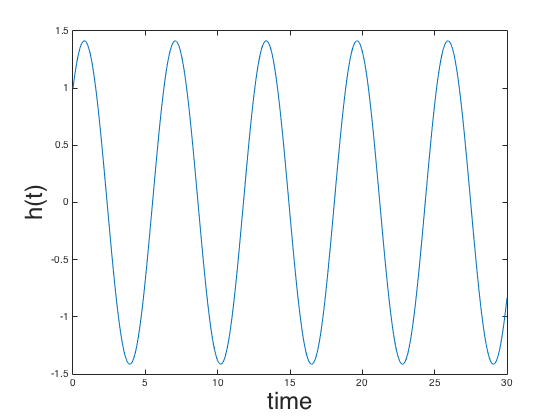
\includegraphics[width=0.5\textwidth, height=0.125\paperheight]{osc_impulse}
   \end{tabular}
  %  \end{center}
      \caption{(Left) Graphical representation of the cell cycle control gene network, and (right) plot of the phenotype $\phi(t)$ against time $t$.} \label{fig:oscillator}
    \end{figure}
  \end{example}


\subsection*{Equivalent gene networks}

As reviewed above,
some systems with identical phenotypes are known to differ, sometimes substantially, at the molecular level; 
systems with identical phenotypes do not necessarily have identical kryptotypes.
How many different mechanisms perform the same function? 

Two systems are equivalent if they produce the same phenotype given the same input,
i.e., have the same input--output relationship.
We say that
the systems defined by $(A,B,C)$ and $(\bar A,\bar B,\bar C)$ are
\textbf{phenotypically equivalent} 
if their impulse response functions are the same:
$h(t) = \bar h(t)$ for all $t \ge 0$.
This implies that for any acceptable input $u(t)$,
if $(\kappa_u(t),\phi_u(t))$ and $(\bar \kappa_u(t),\bar \phi_u(t))$ are the solutions to equation \eqref{eqn:system}
of these two systems, respectively, then
\begin{align*}
      \phi_u(t) = \bar \phi_u(t) \qquad \text{for all} \; t \ge 0.
\end{align*}
% (recall that $\kappa(0) = \bar \kappa(0) = 0$). 


One way to find other systems phenotypically equivalent to a given one
is by change of coordinates:
if $V$ is an invertible matrix, then the systems $(A,B,C)$ and $(VAV^{-1},VB,CV^{-1})$
are phenotypically equivalent because their impulse response functions are equal:
  \begin{equation}
    \begin{aligned}
      h(t) &= C e^{A t} B 
      = C V^{-1} V e^{A t} V^{-1} V B \\
      &= C V^{-1} e^{V A V^{-1} t} V B 
      = \bar{C} e^{\bar{A} t} \bar{B} = \bar h(t).
    \end{aligned}
  \end{equation}
However, not all phenotypically equivalent systems are of this form:
systems can have identical impulse responses without being coordinate changes of each other.
In fact, systems with identical impulse responses can involve interactions between different
numbers of molecules, and thus 
have kryptotypes in
different dimensions altogether.

This implies that most systems have at least $n^2$ degrees of freedom,
where recall $n$ is the number of components of the kryptotype vector.
This is because for an arbitrary $n \times n$ matrix $Z$,
taking $V$ to be the identity matrix plus a small perturbation in the direction of $Z$
above implies that
moving $A$ in the direction of $ZA - AZ$
% (e.g., $\bar A = A + \epsilon(ZA-AZ)$)
while also moving $B$ in the direction of $ZB$ 
and $C$ in the direction of $-CZ$
will leave the phenotype unchanged.
If $A$ is invertible, for instance,
then any such $Z$ will result in a different system.

It turns out that in general, there are more degrees of freedom,
except if the system is \emph{minimal} -- meaning, informally, that it uses the smallest possible number of components
to achieve the desired dynamics.
Results in system theory show that any system can be realized in a particular minimal dimension
(the dimension of the kryptotype, $n_\text{min}$),
and that any two phenotypically equivalent systems of dimension $n_\text{min}$ are related by a change of coordinates.

Some gene networks, however, can grown or shrink, perhaps following gene duplications and deletions, 
and also still preserve their phenotypes.
More generally, even if the system is not minimal, 
results from systems theory % -- the Kalman decomposition --
explicitly describe the set of all phenotypically equivalent systems.
% Could define script S here for 'system' if we want: $\Sys$
We refer to $\allS(A_0,B_0,C_0)$ as the set of all systems phenotypically equivalent
to the system defined by $(A_0, B_0, C_0)$.
Concretely, this is
\begin{equation} \label{eqn:equivalence}
  \begin{aligned}
    \allS(A_0, B_0, C_0) 
      &= \left\{
        (A,B,C) : C e^{At} B = C_0 e^{A_0 t} B_0 \; \text{for}\; t \ge 0 
      \right\}  .
  \end{aligned}
\end{equation}
These systems need not have the same kryptotypic dimension $n$,
but must have the same input and output dimensions ($\ell$ and $m$, respectively).

The Kalman decomposition, which we now describe informally, elegantly characterizes this set
\citep{kalman1963mathematical,kalman1969topics,anderson1966equivalence}.
To motivate this, first note that the input $u(t)$ only directly pushes the system
in certain directions (those lying in the span of the columns of $B$).
As a result, different combinations of input can 
move the system in any direction that lies in what is known as the \emph{reachable subspace}.
Analogously, we can only observe motion of the system in certain directions
(those lying in the span of the columns of $C$),
and so can only infer motion in what is known as the \emph{observable subspace}.
The Kalman decomposition then classifies each direction in kryptotype space
as either reachable or unreachable, and as either observable or unobservable.
Only the components that are both reachable and observable determine the system's phenotype --
that is, components that respond to an input and components that produce an observable output. 
% it is possible to add components that respond to an input, 
% but do not influence the output, or components that, in principle, influence the output, but do not respond to any inputs. 

Concretely, the \textbf{Kalman decomposition} of a system $(A,B,C)$  
gives a change of basis $P$ such that
the transformed system $(PAP^{-1},PB,CP^{-1})$  has the following form:
\begin{align*}
       PAP^{-1}
       &=
       \left[ \begin{array}{cccc}
           A_{\rno} & A_{\rno,\ro} & A_{\rno,\nrno} & A_{\rno,\nro} \\
           0 & A_{\ro} & 0 & A_{\ro,\nro} \\
           0 & 0 & A_{\nrno} & A_{\nrno,\nro} \\
          0 & 0 & 0 & A_{\nro}
       \end{array} \right] ,
\end{align*}
and
\begin{align*}
     PB
     &=
    \left[ \begin{array}{cccc}
         B_{\rno} \\
         B_{\ro} \\
         0 \\
         0 
   \end{array} \right] 
   &
   (CP^{-1})^T
   &=
   \left[ \begin{array}{cccc}
       0 \\
       C_{\ro}^T \\
       0 \\
       C_{\nro}^T
   \end{array} \right] .
\end{align*}
% and
% \begin{align*}
%    CP^{-1}
%    &=
%    \left[ \begin{array}{cccc}
%        0 & C_{\ro} & C_{\nrno} & 0 
%    \end{array} \right] .
%\end{align*}
The impulse response of the system is given by
\begin{align*}
      h(t) = C_{\ro} e^{A_{\ro} t} B_{\ro},
\end{align*}
and therefore, the system is phenotypically equivalent to the \emph{minimal} system $(A_{\ro}, B_{\ro}, C_{\ro})$.
(Here the subscript $\ro$ refers to the both \emph{reachable and observable} subspace,
while $\nrno$ refers to the \emph{unreachable and unobservable} subspace,
and similarly for $\nro$ and $\rno$.)

Any two minimal systems are related by a change of coordinates,
and so the minimal subsystems obtained by the Kalman decomposition
are unique up to a change of coordinates.
In particular, this implies that there is no equivalent system with a smaller number of kryptotypic dimensions
than the dimension of the minimal system.
It is also remarkable to note that the gene regulatory network architecture to achieve a given input--output map is never unique --
both the change of basis used to obtain the decomposition
and, once in this form, all submatrices other than $A_{\ro}$, $B_{\ro}$, and $C_{\ro}$ can be changed without affecting the phenotype,
and so represent degrees of freedom.

\emph{Note on implementation:}
The \emph{reachable subspace},
which we denote by $\reachable$,
is defined to be the closure of $\spn(B)$ under applying $A$,
% (or equivalently, the span of $B, AB, A^2B, \ldots A^{n-1}B$).
% Analogously to this, we define
and the \emph{unobservable subspace}, 
%$\mathcal{O}$, is the closure of $\spn(C^T)$ under applying $A$.
denoted $\unobservable$, is the largest $A$-invariant subspace
contained in the null space of $C$.
% and $\reachable$ is the largest $A$-invariant subspace contained in the image of $B$.)
The four subspaces, $\rno$, $\ro$, $\nrno$, and $nro$
are defined from these by intersections and orthogonal complements.

%Usually, the dimension $n$ and the reference system $\Sys_0$ is implicit and we write only $\calA$.
%Further, we refer to the set of all linear systems with impulse response $h(t)$, regardless of dimension, to be $\allS$,
%  \begin{align}
%    \allS := \bigcup_{n=\min}^{\infty} \calA_n(\Sys_0)
%  \end{align}

For the remainder of the paper, we interpret $\allS$ as the phenotypically neutral landscape, 
wherein a large population will drift under environmental and selective stasis. 
Even if the phenotype is constrained and remains constant through evolutionary time, 
the molecular mechanism underpinning it is not constrained and likely will not be conserved.

Finally, note that if $B$ and $C$ are held constant --
i.e., if the relationships between environment, kryptotype, and phenotype do not change --
there are \emph{still} usually degrees of freedom. 
These correspond to distinct genetic networks that perform indistinguishable functions. 
The following example \ref{ex:all_osc} gives the set of minimal systems equivalent to the oscillator of example \ref{ex:oscillator},
that all share common $B$ and $C$ matrices.


\begin{example}[All Phenotypically Equivalent Oscillators] \label{ex:all_osc}
The oscillator of example \ref{ex:oscillator} is minimal, and so any equivalent system is a change of coordinates
by an invertible matrix $V$.
If we further require $B$ and $C$ to be invariant then we need $VB=B$ and $CV=C$.
Solving these equations,
we find that a one-parameter family $(A(\tau), B, C)$ describes the set of all two-gene systems
phenotypically equivalent to the oscillator,
where
    \begin{align*}
      A(\tau) &= \frac{1}{\tau-1} \begin{bmatrix} \tau & -1 \\ 2 \tau(\tau - 1) + 1 &  -\tau \end{bmatrix} \ \text{for} \ \tau \neq 1 .
    \end{align*}
The resulting set of systems,
and their dynamics, are depicted in Figure \ref{fig:all_osc}
\end{example}


    \begin{figure}[H]
    \centering
\begin{tabular}{cc}
\begin{tikzpicture}
\begin{scope}[every node/.style={circle,thick,draw}]
  \node (A) at (0,0) {$\kappa_{1}$};
    \node[dashed] (B) at (4,0) {$\kappa_{2}$};
    \node[shape=rectangle] (U) at (2,2) {input};
    \node[shape=rectangle] (y) at (2,-2) {output};
\end{scope}

\begin{scope}[>={Stealth[black]},
              every node/.style={fill=white,circle},
              every edge/.style={draw=black, thick}]
    \path [->, sloped] (A) edge[bend left] node {\tiny $2 \tau + (\tau-1)^{-1}$} (B);
    \path [->, sloped] (B) edge[bend left] node {\tiny $-(\tau-1)^{-1}$} (A); 
    \path[->] (U) edge[dashed] node {\tiny $1$} (A);
    \path[->] (U) edge[dashed] node {\tiny $1$} (B);
    \path[->] (A) edge[dashed, bend right] node {\tiny $1$} (y);
\end{scope}
\begin{scope}[>={Stealth[black]},
              every edge/.style={draw=black, thick}]
    \path [->] (A) edge[loop left] node[sloped, anchor=center, above] {\tiny $1 + (\tau-1)^{-1}$} (A);
    \path [->] (B) edge[loop right] node[sloped, anchor=center, above] {\tiny $-1 - (\tau-1)^{-1}$} (B);
\end{scope}
\end{tikzpicture} &	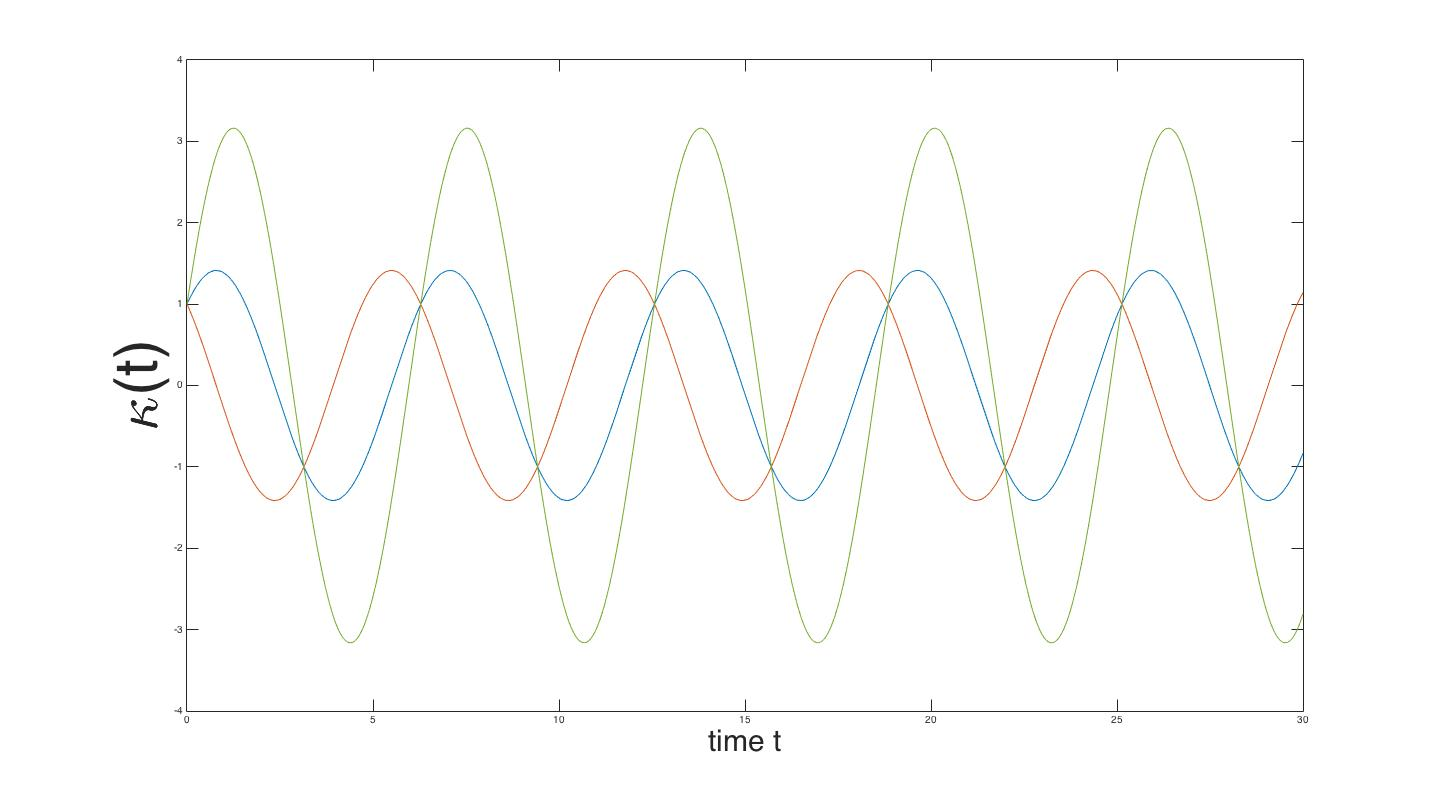
\includegraphics[width=0.5\textwidth, height=0.125\paperheight]{figures/osc_kryp_compare}
    \end{tabular}
% \caption{}
      \caption{
      (Left) $A(\tau)$, the set of all phenotype-equivalent cell cycle control networks.
      (Right) Gene-1 dynamics (blue) for both systems $A(0)$ and $A(2)$ are identical, however, $A(0)$ gene-2 dynamics (orange) differ from $A(2)$ (green).
      % Both gene-1 dynamics are given by $\kappa_{1}(t) = \sin t + \cos t$, and gene-2 by $\kappa_{2}(t) = \cos t - \sin t$ ($A(0)$) and $\kappa'_{2}(t) = \cos t + 3 \sin t$ ($A(2)$).
      } 
    \label{fig:all_osc}
\end{figure}


\paragraph{Sexual reproduction and recombination}
Parents with phenotypically equivalent, yet different, gene networks may produce offspring with dramatically different phenotypes. 
If the phenotypes are significantly divergent then the offspring may be inviable or otherwise have very low fitnesses, 
despite both parents being well adapted. If this is consistent for the entire population, we would consider them to be separate species.

Diploid organisms have two copies of the genome, each of which encodes a set of system coefficients.
We assume that a diploid who has inherited systems $(A', B', C')$ and $(A'', B'', C'')$ from her mother and father, respectively,
has phenotype determined by the system that averages these two,
$((A'+A'')/2, (B'+B'')/2, (C'+C'')/2)$.

Each of the copies of the genome an organism inherits from her parents are generated from their two copies of the genome by meiosis,
in which the diploid parent recombines her two genomes.
We will assume that each coefficient (i.e., entry of $A$, $B$ or $C$)
is determined by a single nonrecombining locus,
so that each coefficient in the system produced by meiosis is an independent random choice
of the two parental coefficients.
With these definitions, an $F_1$ offspring of two individuals
carries one system copy from each parent,
and an $F_2$ is the offspring of two independently formed $F_1$ individuals.
If the parents are from distinct populations,
these are first- and second-generation hybrids, respectively.

This is a simplification:
since the $i^\text{th}$ row of $A$ summarizes how each gene regulates gene $i$,
and hence is determined by the promoter region of gene $i$,
we would actually expect the elements of a row of $A$ to tend to be inherited together.
Similarly, we expect in practice heritable variation in each coefficient
to be determined by more than one locus --
but this may be a reasonable approximation.

The offspring of two systems with the same phenotype may not have the same phenotype as the parents -- in other words $\allS$, the set of all systems phenotypically equivalent to a given one, is not, in general, closed under averaging or recombination.
Next we discuss how this fact can contribute to hybrid incompatibility and genetic load.
If sexual recombination among systems drawn from $\allS$ yields systems with divergent phenotypes, populations containing significant diversity in $\allS$ can carry genetic load, and isolated populations may fail to produce hybrids with viable phenotypes.


\begin{figure}[H]
\centering
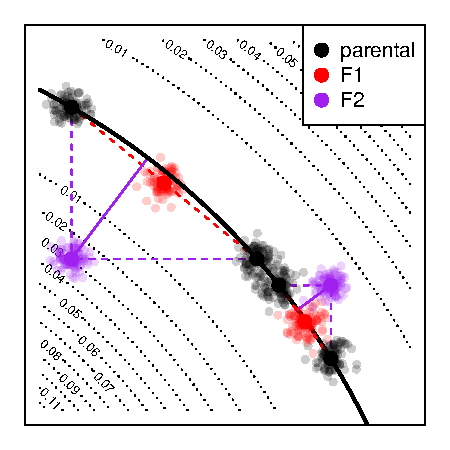
\includegraphics{figures/conceptual_fig}
\caption{
    \label{fig:conceptual_fig}
    A conceptual figure of the fitness consequences of hybridization:
    axes represent system coefficients (i.e., entries of $A$);
    the line of optimal system coefficients is down in black;
    dotted lines give phenotypic distances to the optimum.
    Two pairs of parental populations are shown in black, along the optimum;
    a hypothetical population of $F_1$s are shown for each in red,
    and the distribution of one type of $F_2$ is shown in purple
    (other types of $F_2$ are not shown).
    Solid lines depict the distance of the $F_2$ to optimum.
}
\end{figure}

\paragraph{Hybrid incompatibility}
Two parents with the optimal phenotype can produce offspring whose phenotype is suboptimal
if the parents have different underlying systems.
This leads to the question: 
How quickly does the hybrid phenotype break down with increasing distance between the parents?
To quantify this, we will measure how far a system's phenotype is from optimal
using a weighted difference between impulse response functions.
Suppose that $\rho(t)$ is a nonnegative, smooth, square-integrable weighting function,
suppose that $h_0(t)$ is the \emph{optimal} impulse response function 
and define the ``distance to optimum'' of another impulse response function
to be
\begin{align}
\label{eqn:distance}
	D(h) = \left( \int_0^\infty \rho(t) \|h(t) - h_0(t)\|^2 dt \right)^{1/2} .
\end{align}
Consider reproduction between a parent with system $(A, B, C)$ 
and another displaced by distance $\epsilon$ in the direction $(X,Y,Z)$,
i.e., having  system $(A + \epsilon X, B + \epsilon Y, C + \epsilon Z)$.
We assume both are ``perfectly adapted'' systems, 
i.e., having impulse response function $h_0(t)$,
and their offspring has impulse response function $h_\epsilon(t)$.
A Taylor expansion of $D(h_\epsilon)$ in $\epsilon$ is explicitly worked out in Appendix \ref{apx:H_calc},
and shows that the phenotype of an $F_1$ hybrid between these two is at distance proportional to $\epsilon^2$ from optimal,
while $F_2$ hybrids are at distance proportional to $\epsilon$.
This is because an $F_1$ hybrid has one copy of each parental system,
and therefore lies directly between the parental systems (see Figure \ref{fig:conceptual_fig}) --
the parents both lie in $\allS$, which is the valley defined by $D$,
and so their midpoint only differs from optimal due to curvature of $\allS$.
In contrast, an $F_2$ hybrid may be homozygous for one parental type in some coefficients
and homozygous for the other parental type in others;
this means that each coefficient of an $F_2$ may be equal to either one of the parents,
or intermediate between the two;
this means that possible $F_2$ systems may be as far from the optimal set, $\allS$,
as the distance between the parents.
The precise rate at which the phenotype of a hybrid diverges depends on the geometry --
in Figure \ref{fig:conceptual_fig}, this is depicted as the angle of the black line (the optimal set)
with respect to the coordinates.


\begin{example}[Hybrid Incompatibility in the Oscillator] \label{ex:hybrid_osc}
Offspring of two equivalent systems from Example \ref{ex:all_osc}
can easily fail to oscillate.
For instance, the $F_1$ offspring between homozygous parents at $\tau=0$ and $\tau=2$
has phenotype $\phi_{F_1}(t) = e^t$, rather than $\phi(t) = \sin t + \cos t$.
However, the coefficients of these two parental systems differ substantially,
probably more than would be realistically observed between diverging populations.
In figure \ref{fig:hybs} we compare the phenotypes for $F_1$ and $F_2$ hybrids between more similar parents,
and see increasingly divergent phenotypes as the difference between the parental systems increases.
(In this example, the coefficients of $A(2+\epsilon)$ differ from those of $A(2)$ by an average factor of $1+\epsilon/2$;
such small differences could plausibly be caused by changes to promoter sequences.)
This divergence is quantified in Figure \ref{fig:osc_incompat},
which shows that mean distance to optimum phenotype of the $F_1$ and $F_2$ hybrid offspring between $A(2)$ and $A(2+\epsilon)$
increases with $\epsilon^2$ and $\epsilon$, respectively.

The coefficients in $A$ -- i.e., the regulatory coefficients --
differ between parents by only a few percent (around 0.5\% for $\tau=2.01$ and 5\% for $\tau=2.1$).
This is well within the amount of regulatory coefficient variation we expect to find segregating within real populations
(discussed further below). 
For these small values of $\epsilon$, hybrid phenotypes remain relatively stable, 
consistent with the idea that natural selection will allow such intrapopulation variation. 

%%% figure of tau=0 and tau=2 hybrid:
%  \begin{figure}[H] 
%    \centering
%    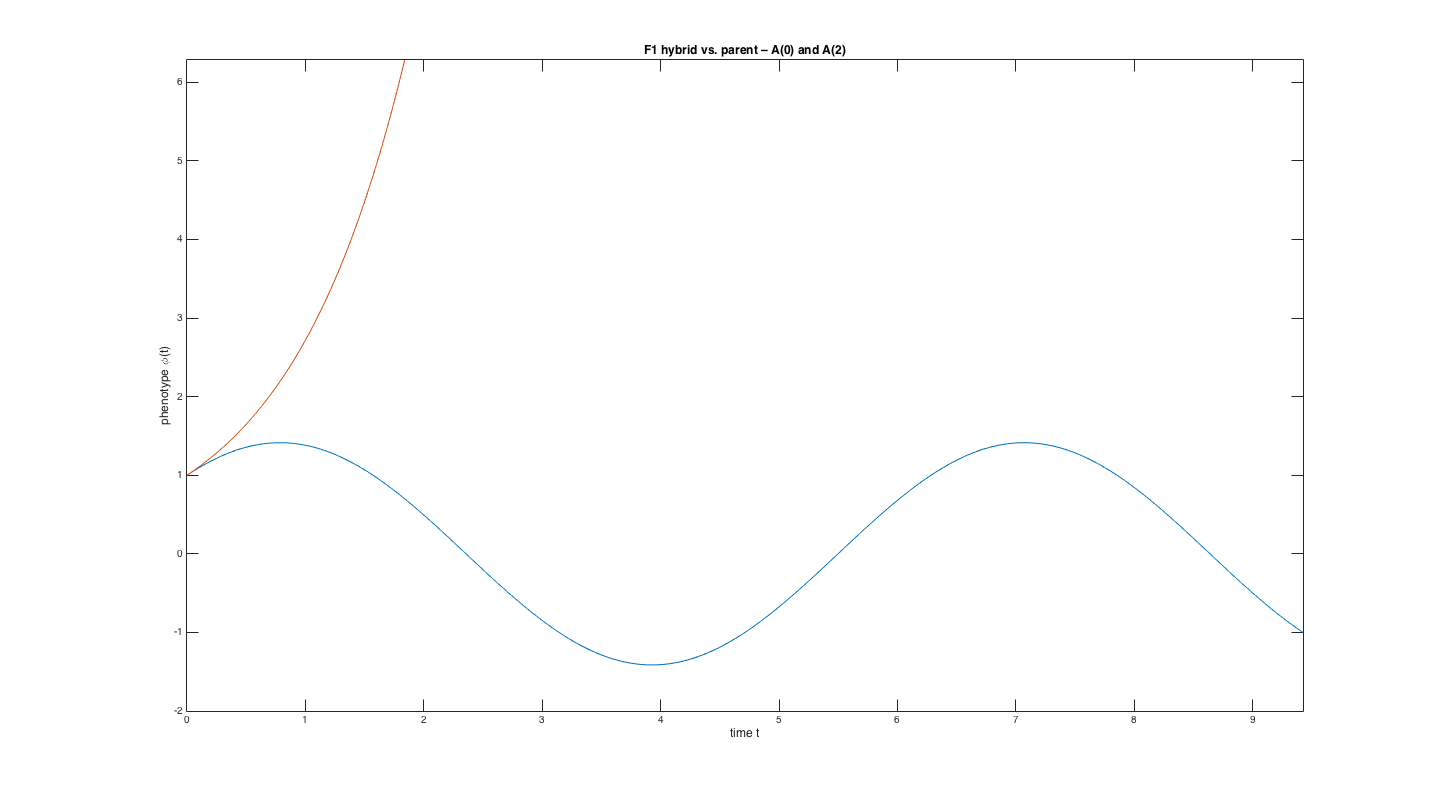
\includegraphics[width=0.5\textwidth, height=0.125\paperheight]{expF1}
%    \caption{\textbf{Hybrid phenotypic breakdown} $F_1$ hybrid (orange) and parental (blue) phenotypic cell-cycle control (oscillator) dynamics %for an $\Sys(0)$ by $\Sys(2)$ cross from Example \ref{ex:all_osc}. The $F_1$ hybrid
%$\left(A_{F_1}\!\!=\!\!\tfrac{A\!(\!0\!) \! + \! A\!(\!2\!)}{2}\right)$
%gene expression fails to oscillate and instead grows exponentialy
%($\phi_{F_0}\! = \! \sin t \! + \! \cos t$, however $\phi_{F_1} \! = \! e^t$).
%    }
%    \label{fig:expF1}
%  \end{figure}


\begin{figure}[H]
  \centering
  \begin{tabular}{ccc}
    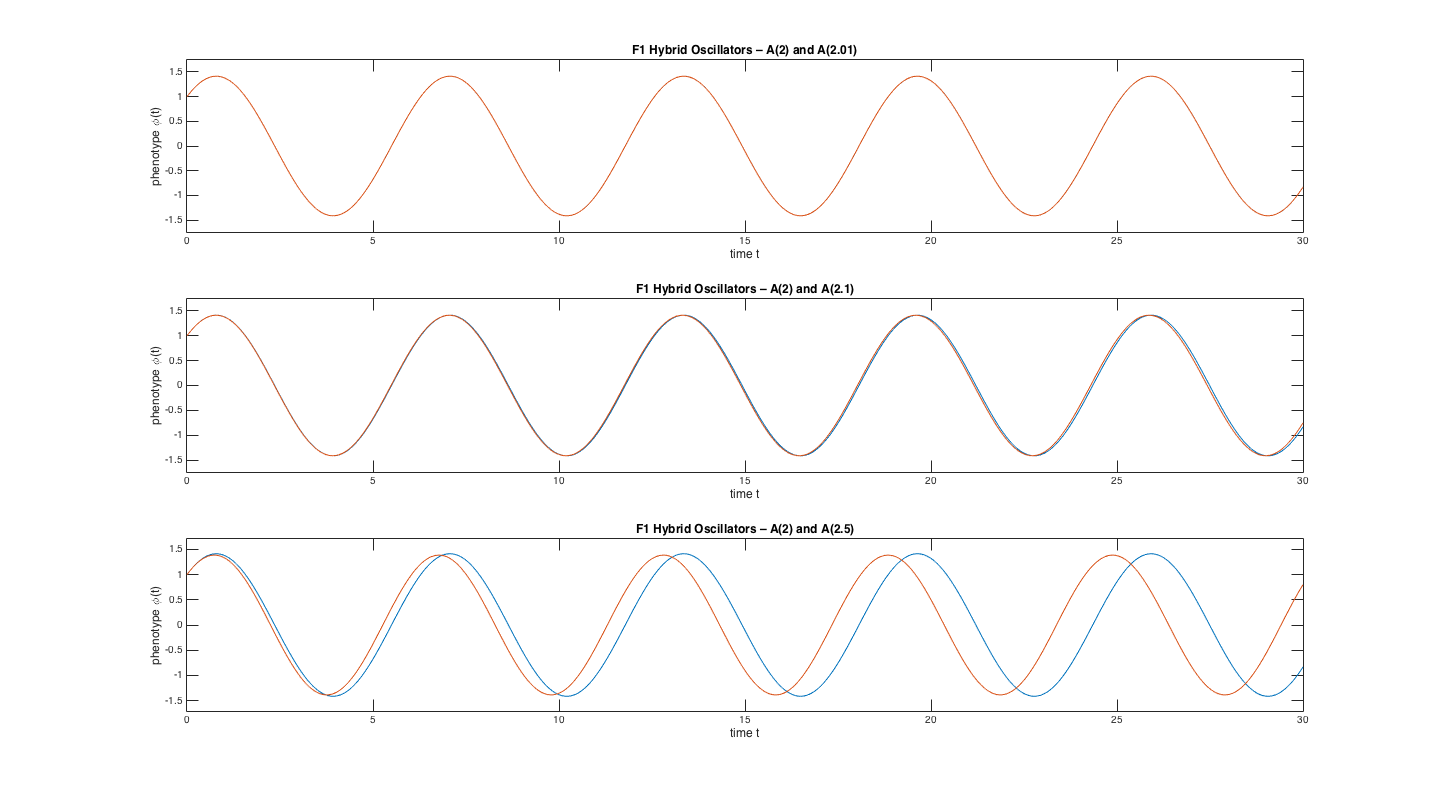
\includegraphics[width=0.5\textwidth, height=0.25\paperheight]{F1_comparison} &
    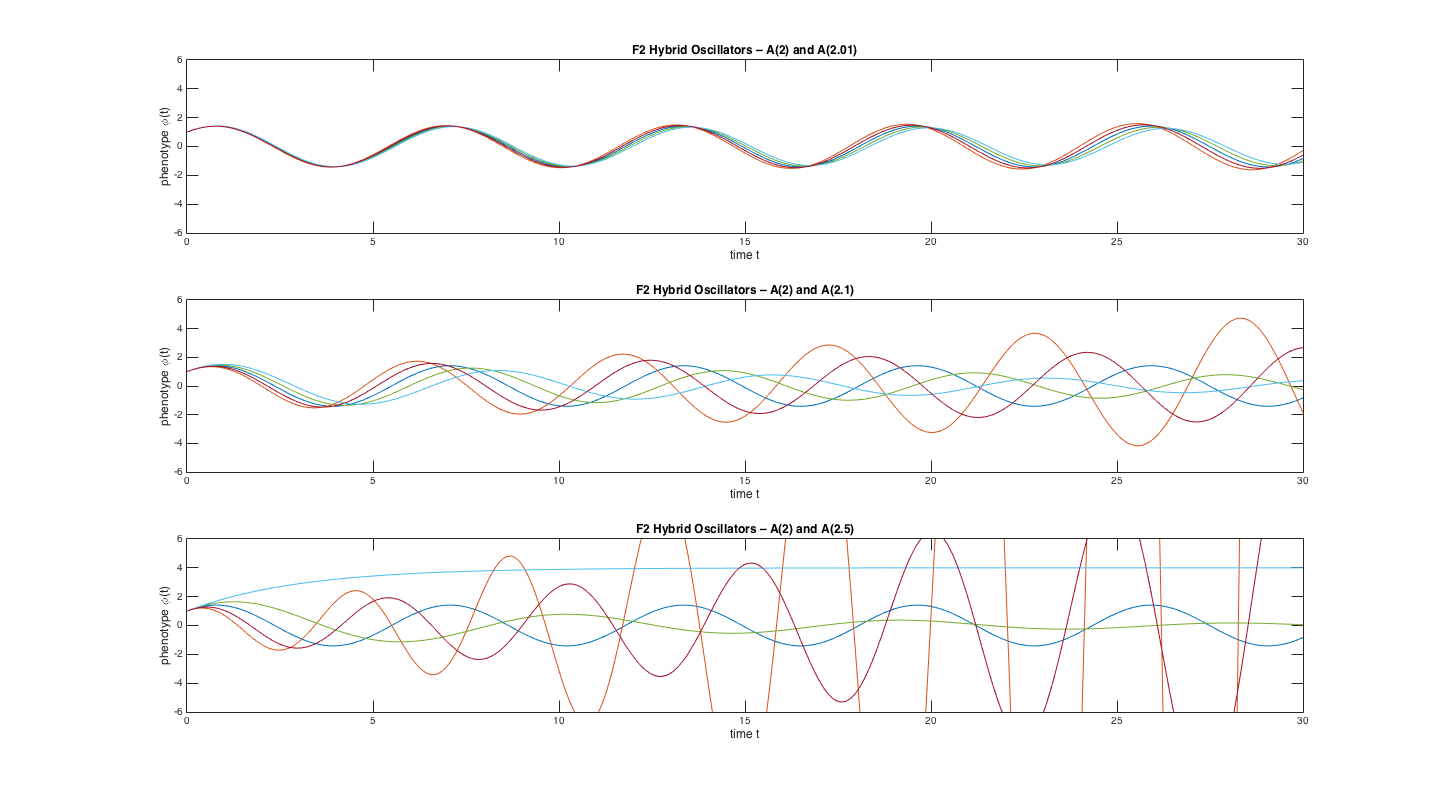
\includegraphics[width=0.5\textwidth, height=0.25\paperheight]{F2s_comparison2}
  \end{tabular}
  \caption{
  \textbf{(left)} Phenotypes of $F_1$ hybrids between an $A(2)$ parent and, top-to-bottom, an $A(2.01)$, an $A(2.1)$, and $A(2.5)$ parent.
    Parental phenotypes ($\sin t + \cos t$) are shown in blue, and hybrid phenotypes in orange.
    \textbf{(right)} Phenotypes of $F_2$ hybrids between the same set of parents,
    with parental phenotype again in blue.
    Different lines correspond to different $F_2$s produced by recombination;
    note that some completely fail to oscillate.
    \plri{make axis labels bigger}
  } \label{fig:hybs}
\end{figure}

  \begin{figure}[H]
  \label{fig:osc_incompat}
    \centering
    \begin{tabular}{cc}
    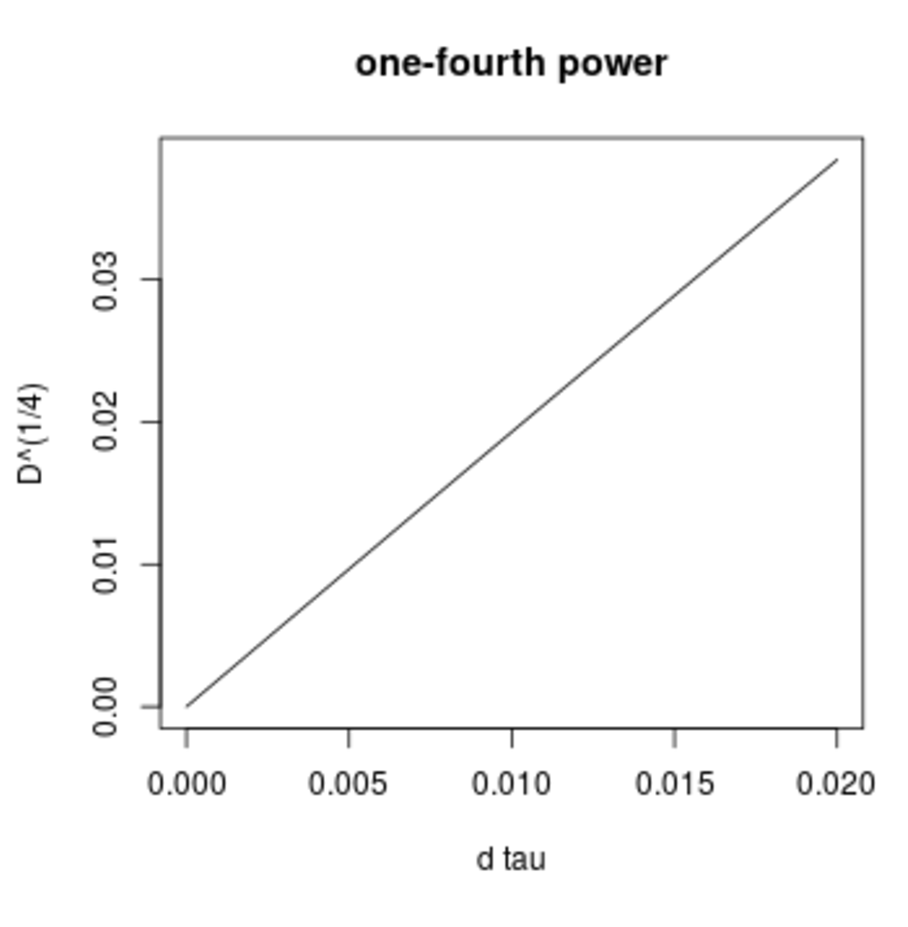
\includegraphics[width=0.4\textwidth]{figures/f1_quartic2} &
    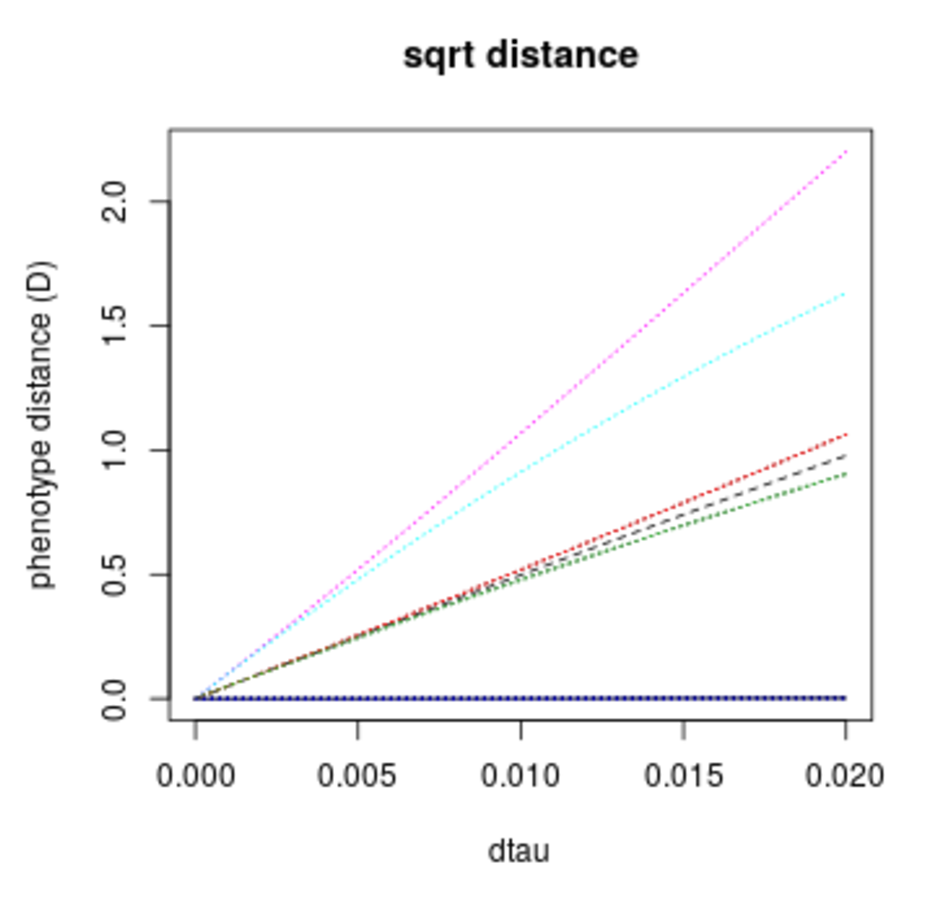
\includegraphics[width=0.4\textwidth]{figures/f2_quad2}
    \end{tabular}
    \caption{
    \textbf{(left)} Phenotype distance to optimum, $D$, using $\rho(t) = \exp(-t/4\pi)$
    for $F_1$ hybrids between an $A(2)$ and an $A(2+\epsilon)$ parent.
    \textbf{(right)} Same, but for $F_2$ offspring (one line per type of $F_2$).
    \plri{make this $D$ not $D^2$ and say which line is the overall average $F_2$.}
    } \label{fig:osc_incompat}
  \end{figure}
\end{example}

\paragraph{Haldane's rule}
This model naturally predicts
Haldane's rule, the observation that if only one hybrid sex is sterile or inviable 
it is likely the heterogametic sex (e.g., the male in XY sex determination systems) \citep{haldane1922sex}.
For example, consider an XY species with a two-gene network where the first gene resides on an autosome and the second gene on the X chromosome.
A male whose pair of haplotypes are 
$\left( \left[ \begin{smallmatrix} A_1 & A_2 \\ \cdot & \cdot \end{smallmatrix} \right], \left[ \begin{smallmatrix} A_1 & A_2 \\ X_1 & X_2 \end{smallmatrix} \right] \right)$
has phenotype determined by $A = \left[ \begin{smallmatrix} A_1 & A_2 \\ X_1/2 & X_2/2 \end{smallmatrix} \right]$,
while a female homozygous for the haplotype
$\left[\begin{smallmatrix} \bar A_1 & \bar A_2 \\ \bar X_1 & \bar X_2 \end{smallmatrix}\right]$,
thanks to X-inactivation, has phenotype determined by
$A = \left[\begin{smallmatrix} \bar A_1 & \bar A_2 \\ \bar X_1/2 & \bar X_2/2 \end{smallmatrix}\right]$.
An $F_1$ male offspring of these two will have phenotype determined by
$\frac{1}{2} \left[\begin{smallmatrix} A_1 + \bar A_1 & A_2 + \bar A_2 \\ \bar X_1 & \bar X_2 \end{smallmatrix}\right]$.
If both genes resided on the autosomes this system would only be possible in an $F_2$ cross.
More generally, 
if the regulatory coefficients for a system are shared between the sex and one or more autosomal chromosomes, 
$F_1$ males are effectively equivalent to purely autosomal-system $F_2$s.

This mechanism is apparently distinct from the currently favored ``dominance'', ``faster-X'', and ``faster-male'' theories \citep{orr1997haldane, coyne1998evolutionary} to explain Haldane's rule,
and makes several different predictions than the dominance theory as formulated by \citet{turelli1995dominance}.
\plr{what are they?}
\citet{turelli1995dominance} employ a population genetic model which strictly requires alleles causing hybrid incompatibility on the X chromosome not to exhibit additive effects, that is the \emph{dominance coefficient} (typically $h$ in classic population genetics) must not be equal to $\frac{1}{2}$. In their model, if alleles are strictly additive, that is neither dominant nor recessive, then male and female $F_1$ hybrids will drop in fitness at the exact same rates, and therefore defy Haldane's rule. 
Furthermore, the dominance theory struggles with dosage compensation and X-inactivation \citep{watson2012haldane}; the present model, however, complies with Haldane's rule with X-inactivation explicitly included.

%%%%%%%%%%%%%%%%%%%%%%%%
\section*{System drift and the accumulation of incompatibilities}

Thus far we have shown that many distinct molecular mechanisms can realize identical phenotypes
and that these mechanisms may fail to produce viable hybrids.
This begs the question: does evolution shift molecular mechanisms
fast enough to be a significant driver of speciation?
To approach this question,
we explore a general quantitative genetic model in which a population drifts stochastically
near a set of equivalent and optimal systems
due to the action of recombination, mutation, and demographic noise.
Although this is motivated by the results on linear systems above,
the quantitative genetics calculations are more general,
and only depend on the presence of genetic variation and a continuous set of phenotypically equivalent systems.

We will suppose that each organism's phenotype is determined by her vector of coefficients, denoted by $x=(x_1, x_2, \ldots, x_L)$,
and that the corresponding fitness is determined by the distance of her phenotype to optimum.
The optimum phenotype is unique, but is realized by many distinct $x$ -- those falling in the ``optimal set'' $\allS$.
The phenotypic distance to optimum of an organism with coefficients $x$ is denoted $D(x)$.
In the results above, $x = (A,B,C)$ and $D(x)$ is given by equation \eqref{eqn:distance}.
determines a system (this is a system $(A,B,C)$ above) 
with fitness determined by its phenotypic distance $D(x)$ from an optimum (this is analogous to $\allS$ above). 
Concretely, we define the fitness at $x$ to be $\exp(-D(x)^2)$.
% this assumption does not entail a loss of generality since $D$ is arbitrary.
We will assume that in the region of interest, the map $D$ is smooth
and that we can locally approximate the optimal set $\allS$ as a quadratic surface.
As above, an individual's coefficients are given by averaging her parentally inherited coefficients and adding random noise due to segregation. 
Concretely, we use the \emph{infinitesimal model} for reproduction \citep{barton_infinitesimal} --
the offspring of parents at $x$ and $x'$ will have coefficients $(x+x')/2 + \varepsilon$,
where $\varepsilon$ is a Gaussian displacement due to random assortment of parental alleles.

\paragraph{System drift}
% plr how fast does it drift
We work with a randomly mating population of effective size $N_e$. 
If the regulatory coefficient population variation
has standard deviation $\sigma$ in a particular direction,
since subsequent generations resample from this diversity,
the population mean coefficient will move a random distance of size $\sigma/\sqrt{N_e}$ per generation,
simply because this is the the standard deviation of the mean of a random sample \citep{lande_drift}.
% (This could be taken as a definition of $N_e$.)
Selection will tend to restrain this motion,
but movement along the optimal set $\allS$ is unconstrained,
and so we expect the population mean to drift along the optimal set like a particle diffusing.
% (although perhaps complicated by recombination load \citep{recomb_load})
The amount of variance in particular directions in coefficient space 
depends on constraints imposed by selection and 
correlations between the genetic variation underlying different coefficients (the $G$ matrix \citep{G_matrix}).
It therefore seems reasonable to coarsely model the time evolution of population variation in regulatory coefficients as 
a ``cloud'' of width $\sigma$ about the population mean, 
which moves as an unbiased Brownian motion through the set of network coefficients that give the optimal phenotype.

% covariance which may arise due to functional constraints and/or statistical linkage.
% There may well be functional constraints -- but these are not sufficiently well-known to say anything general about.
%For instance,
%if the variation is due to \textit{cis}-regulatory variants,
%the genetic basis of each \emph{row} of $A$ likely lies within a few kilobases of tightly linked sequence,
%across which a population may carry only a few common haplotypes.
%However, covariance due to transiently assembled haplotypes is not expected to be stable over long periods of time --
%a common \textit{cis}-regulatory haplotype of transcription factor $k$ with particularly strong binding to both $i$ and $j$
%(leading to positive covariance between $A_{ik}$ and $A_{jk}$)
%is no more likely to appear than one with strong binding to $i$ but particularly weak binding to $j$ (negative covariance).
%(Such transient covariances may well increase the variance of the per-generation change in network mean, however \citep{barton_linkage}.)

There will in general be different amounts of variation in different directions;
to keep the discussion intuitive, we only discuss $\sigma_N$, the amount of variation in ``neutral'' directions
(i.e., directions along $\allS$),
and $\sigma_S$, the amount of variation in ``selected'' directions (perpendicular to $\allS$).
The other relevant scale we denote by $\gamma$,
which the scale on which distance to phenotypic optimum changes as $x$ moves away from the optimal set, $\allS$.
Concretely, $\gamma$ is
%the inverse of the derivative of 
$1/(\frac{d}{du}D(x+uz))$ 
with respect to $u$ where $x$ is optimal and $z$ is a ``selected'' direction perpendicular to $\allS$.
With these parameters, a typical individual will have a fitness of around $\exp(-(\sigma_S/\gamma)^2)$.
Of course, there are in general many possible neutral and selected directions;
we take these values to be representative of the possible directions.

\paragraph{Hybridization}
The means of two allopatric populations each of effective size $N_e$ separated for $T$ generations
will be a distance roughly of order $2\sigma_N \sqrt{T/N_e}$ apart along $\optx$.
(Consult figure \ref{fig:conceptual_fig} for a conceptual diagram.)
A population of $F_1$ hybrids has one haploid genome from each,
whose coefficients are averaged,
and so will have mean system coefficients at the midpoint between their means.
Each $F_2$ hybrid will be homozygous for one parental allele on average at half of the loci in the genome,
so the distribution of $F_2$s will have mean at the average of the two populations,
but will have higher variance.
The variance of $F_2$s can be shown to increase linearly with the square of the distance between
parental population means
under models of both simple and polygenic traits.
This is suggested by figure \ref{fig:conceptual_fig} and shown in Appendix \ref{apx:seg_cov}.
\plr{connect to Barton etc polygenic adaptation lit}
Concretely, we expect the population of $F_1$s to have variance $\sigma^2_S$ in the selected direction
(the same as within each parental population),
but the population of $F_2$s will have variance of order $\sigma^2_S + 4 \omega \sigma^2_N T/N_e$,
where $\omega$ is a factor that depends on the genetic basis of the coefficients.
In a model of $p$ traits in which the optimal set $\allS$ has dimension $q$,
% if each trait is controlled by a single locus, $\omega = XXX$,
using the polygenic model of appendix \ref{apx:seg_cov}, $\omega = (p-q)/8$.
If each trait is controlled by a single locus, as in figure \ref{fig:conceptual_fig},
the value is similar.

%%% CITE SOME OF THESE
%% empirical data on sigma
% The amount and structure of this standing variation is established over long time scales
% by many factors, including mutation-selection balance, 
% shifts in the phenotypic optimum, and/or spatial variation in the optimum \citep{hansen1996translating}.
% Quantitative genetics models of mutation-selection balance 
% predict precise levels and structure of standing variation \citep{kimura_mutsel,lande_mutsel,lande1981models},
% but it is unclear how well these predictions match reality \citep{johnson_barton}
% and how much they are expected to change over time \citep{arnold_changing_G}.

What are the fitness consequences?
A population of $F_2$s will begin to be substantially less fit than the parentals
once they differ from the optimum by a distance of order $\gamma$,
i.e., once $\sqrt{4 \omega T/N_e} \approx \gamma / \sigma_N$.
This implies that hybrid incompatibility among $F_2$s should appear on a time scale of 
$N_e (\gamma / \sigma_N)^2 / (4 \omega)$ generations.
The $F_1$s will not suffer fitness consequences until the hybrid mean is further than $\gamma$ from the optimum;
as shown in appendix \ref{apx:away_from_opt} (and suggested by figure \ref{fig:conceptual_fig}),
this deviation of the mean from optimum grows with the square of the distance between the parental populations,
and so we expect fitness costs in $F_1$s to appear on a time scale of $N_e^2$ generations.

% If a population has a Gaussian distribution of trait values with variance $\sigma^2$
% and fitness decays as $\exp(-x^2/2\gamma)$ away from the population mean,
% then the population mean fitness is 
% \begin{align*}
%    \int \frac{1}{\sigma \sqrt{2\pi}} e^{-\frac{x^2}{2\sigma^2}} e^{-\frac{x^2}{2\gamma^2}} dx
%    &=
%    \sqrt{\frac{1}{1 + (\sigma/\gamma)^2}}  \le \frac{1}{\sigma/\gamma} .
% \end{align*}
% If $\sigma$ is much smaller than $\gamma$, the fitness consequences of variation
% (i.e., genetic load) are small,
% but if $\sigma$ is of order $\gamma$, then mean fitness is inversely proportional to trait variance
% (i.e., $\gamma/\sigma$).
% This implies that we expect $\sigma_S < \gamma$
% but that once $T$ is of order $N_e (\gamma / \sigma_H)^2$, there will be loss of fitness
% in $F_2$ hybrids.
% Said another way,
% if we write $\mathcal{F}(T)$ as the mean fitness of an $F_2$ hybrid between two populations separated by $T$ generations,
% then fitness drops with the square root of $T$, measured in units of $N_e$ generations:
% \begin{align*}
%    \mathcal{F}(T) \le \frac{1}{\sigma_H/\gamma}\sqrt{\frac{N_e}{T}} .
% \end{align*}

For a more concrete prediction, suppose that the distribution among hybrids is Gaussian.
A population whose trait distribution is Gaussian with mean $\mu$ and variance $\sigma$,
has mean fitness 
\begin{align} \label{eqn:gauss_fit}
\int_{-\infty}^\infty \frac{1}{\sigma\sqrt{2\pi}} e^{-\frac{(x-\mu)^2}{2\sigma^2}} e^{-\frac{x^2}{2\gamma^2}} dx
&=
\sqrt{\frac{1}{1 + \sigma^2/\gamma^2}} \exp\left\{-\frac{\mu^2}{\gamma^2}\left(\frac{1}{1 + \sigma^2/\gamma^2}\right)\right\} .
% &\approx
% \frac{1}{\sigma/\gamma}\left(1 - \frac{\mu^2}{\gamma^2}\right) .
\end{align}
This assumes a single trait, for simplicity; the multivariate case is done in appendix \ref{apx:gauss_load}.
A population of $F_2$s will have, as above, variance $\sigma^2 = \sigma^2_S + 4 \omega \sigma^2_N T/N_e$.
The mean diverges with the square of the distance between the parentals
with a speed depending on the local geometry of the optimal set
(calculated in appendix \ref{apx:H_calc}), so we set $\mu = c_\mu \gamma T/N_e$.
The mean fitness in parental populations is as in equation \ref{eqn:gauss_fit} with $\mu=0$ and $\sigma = \sigma_S$.
This implies that if we define $\fit_2(T)$ to be the mean relative fitness among $F_2$ hybrids
between two populations separated by $T$ generations, 
(i.e., the mean fitness divided by the mean fitness of the parents)
then
\plr{figure out how dimensions come in here}
\begin{align} \label{eqn:fit2}
\fit_2(T) = 
  \left(1 + \frac{4 \omega (\sigma_N/\gamma)^2}{(1 + (\sigma_S/\gamma)^2)} \frac{T}{N_e} \right)^{-1/2} 
     \exp\left\{-\left(c_\mu \frac{T}{N_e}\right)^2 \left(\frac{1}{1 + (\sigma_S/\gamma)^2 + 4 \omega (\sigma_N/\gamma)^2 T/N_e}\right)\right\} .
\end{align}
If each of the $q$ selected directions acts independently,
the drop in fitness will be $\fit_2(T)^q$
(the expression for the correlated cases is given in Appendix \ref{apx:gauss_load}).
We discuss the implications of this expression in the next section.


%%%%%%%%%%
\paragraph{Speciation rates under neutrality}
Above, equation \eqref{eqn:fit2} shows how fast hybrids become inviable 
as the time that the parental populations are isolated increases;
what does this tell us about speciation rates under neutrality?
From equation \eqref{eqn:fit2} we can observe that
time is always scaled in units of $N_e$ generations,
the population standard deviations are always scaled by $\gamma$,
and the most important term is the rate of accumulation of segregation variance,
$4 \omega (\sigma_N/\gamma)^2$.
All else being equal, this process will lead to speciation more quickly in smaller populations
and in populations with more neutral genetic variation (larger $\sigma_N$).
These parameters are related -- larger populations generally have more genetic variation --
but since these details depend on the situation, we leave these separate.

How does this prediction depend on the system size and constraint?
If there are $p$ trait dimensions, constrained in $q$ dimensions,
and if $\omega$ is proportional to $p-q$,
% the rate that hybrid variance increases with separation between parentals, $\omega$,
% is in some cases proportional to $p-q$, 
then the rate that $F_2$ fitness drops is, roughly,
$(1 + 4 (p-q) C T/n_e)^{-q/2} \propto q (p-q)$, where $C$ is a constant.
This suggests that both degree of constraint and number of available neutral directions
affect the speed of accumulation of incompatibilities.
However, note that in real systems, it is likely that $\gamma$ also depends on $p$ and $q$.
\plr{revisit with sims}

% simgaN = sigmaS = gamma, large population
Suppose in a large, genetically diverse population,
the amount of heritable variation in the neutral and selected directions are roughly equal 
($\sigma_N \approx \sigma_S$)
but the overall amount of variation is (weakly) constrained by selection
($\sigma_N \approx \gamma$).
If so, then the first term of equation \eqref{eqn:fit2} is
$1/\sqrt{1 + 2 \omega T/N_e} \approx 1 - \omega T/N_e$.
If also $\omega=1$, then, for instance, after $0.1 N_e$ generations
the average $F_2$ fitness has dropped by 10\% relative to the parentals.

%  $\sigma_N \approx \sigma_S \ll \gamma$, ``isolated population''
Consider instead a much smaller, isolated population
whose genetic variation is primarily constrained by genetic drift,
so that $\sigma_N \approx \sigma_S \ll \gamma$.
Setting $a = (\sigma_N/\gamma)^2$ to be small,
the fitness of $F_2$s is $\fit_2 \le 1/\sqrt{1 + 4 \omega a T/N_e} \approx 1 - 2 \omega a T/N_e$.
Hybrid fitness seems to drop more slowly in this case in figure \ref{fig:speciation_rates},
but since time is scaled by $N_e$, so speciation may occur \emph{faster} than in a large population.
However, at least in some models \citep{bartonXXX}, in small populations at mutation-drift equilibrium
the amount of genetic variance ($\sigma_N^2$) is proportional to $N_e$,
which would compensate for this difference, 
perhaps even predicting the rate of decrease of hybrid fitness to be \emph{independent} of population size
for small populations.

% $\sigma_N \gg \sigma_S \approx \gamma$, if $N_e$ is big and there's a lot of recombination load (``species complex'')
In the other direction, consider large metapopulations (or isolated ``species complexes'')
among which heritable variation is strongly constrained by selection
(i.e., there is substantial recombination load),
so that $\sigma_S \approx \gamma$ but $\sigma_N/\gamma$ is large.
Then the fitness of $F_2$s is $\fit_2 \le 1/\sqrt{1 + 2 \omega a T/N_e} \approx 1 - \omega a T/N_e$,
and could be extremely rapid if $a$ is large.

For instance, in a population of one million organisms that has 10 generations per year (a drosophilid species, perhaps)
under the ``large population'' scenario of Figure \ref{fig:speciation_rates}A,
system drift would lead to a substantial fitness drop of around 10\% in $F_2$ hybrids in only 10,000 years.
This drop may be enough to induce evolutionary reinforcement of reproductive isolation.
If one thousand of these organisms is isolated (perhaps on an island, as in Figure~\ref{fig:speciation_rates}B),
then a similar drop could occur in around 120 years.
On the other hand, if the population is one of several of similar size
that have recently come into secondary contact after population re-expansion,
the situation may be similar to that of Figure~\ref{fig:speciation_rates}C with $N_e = 10^6$,
the same drop could occur after 1,100 years.
However, hyperdiverse populations of this type may not be stable on these time scales.


\begin{figure}[H]
\label{fig:speciation_rates}
\begin{center}
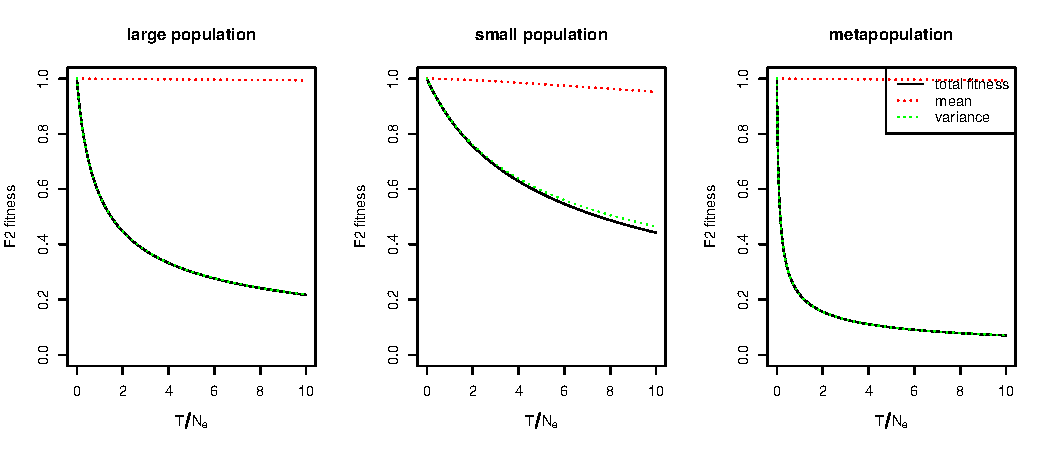
\includegraphics{speciation_rates}
\caption{
Mean drop if $F_2$ fitness relative to parental species,
with $\omega=1$ and 
\textbf{(A)} $\sigma_N^2 = \sigma_S^2 = \gamma^2$
\textbf{(B)} $\sigma_N^2 = \sigma_S^2 = 0.1 \gamma^2$
\textbf{(C)} $0.1 \sigma_N^2 = \sigma_S^2 = \gamma^2$.
The total fitness is from equation \eqref{eqn:fit2},
and is the product of the ``shift of mean'' and ``increase of variance'' terms
(the exponential and the square root, respectively).
Note that, as we assume, the contribution of the shift in mean
is small relative to that of increased variance.
\label{fig:speciation_rates}}
\end{center}
\end{figure}


\subsection*{Genetic variation in empirical regulatory systems}

What is known about the key quantity above, the amount of heritable variation in real regulatory networks?
%These are known at best only roughly \citep{felsenstein1988phylogenies},
%so we aim for order-of-magnitude estimates.
The coefficient $A_{ij}$ from the system \eqref{eqn:system} measures how much the rate of net production of $i$ changes
per change in concentration of $j$.
It is generally thought that regulatory sequence change contributes much more to inter- and intraspecific variation
than does coding sequence change affecting molecular structure \citep{schmidt2010vertebrate}.
In the context of transcription factor networks this may be affected 
not only by the binding strength of molecule $j$ to the promoter region of gene $i$
but also the effects of other transcription factors (e.g., cooperativity)
and local chromatin accessibility \citep{stefflova2013cooperativity}.
For this reason, 
the mutational target size for variation in $A_{ij}$ may be much larger than the dozens of base pairs
typically implicated in the handful of binding sites for transcription factor $j$ of a typical promoter region,
and single variants may affect many entries of $\Sys$ simultaneously.
% (Recall that although these are best modeled through nonlinear terms,
% by linearizing we essentially consider first-order effects.)
% On the other hand, a diverse set of buffering mechanisms are thought to contribute to phenotypic stability
% in the presence of substantial molecular noise \citep{canalization,buffering},
% suggesting that substantial variation in the micro-scale dynamics we consider here
% may be necessary to produce relevant phenotypic effects downstream.

Variation in binding site occupancy may overestimate variation in $A$,
since it does not capture buffering effects (if for instance only one site of many needs be occupied for transcription to begin),
and variation in expression levels measures changes in steady-state concentration (our $\kappa_i$) rather than the \emph{rate} of change.
Nonetheless,
\citet{kasowski2010variation} found differential occupancy in 7.5\%
of binding sites of a transcription factor (p65) between human individuals.
\citet{verlaan2009targeted} showed that cis-regulatory variation
accounts for around 2--6\% of expression variation in human blood-derived primary cells,
while \citep{lappalainen2013transcriptome} found that human population variation 
explained about 3\% of expression variation.
%%\plr{Get some data from at least one other species in here!}
Taken together, this suggests that variation in the entries of $\Sys$
may be on the order of at least a few percent between individuals of a population --
doubtless varying substantially between species and between genes.

The impact of regulatory variation ($\sigma$) above
depends only on its magnitude relative to selection ($\gamma$),
but it seems reasonable that these two quantities are of the same magnitude.


%%%%%%%%%%%%%%%%%%%%%%%%
%%%%%%%%%%%%%%%%%%%%%
\section*{Discussion}

%%% OUTLINE
% - Summarize methods and main result on rate of speciation.
% - What empirical evidence is there that this is actually happening? 
%   * incompats due to misregulation (Noor, Witkopp...)
%   * numerous species that are visually indistinguishable (skinks, ferns)
%   * maybe also ref phylogenetic lit
% - What other evidence could be collected?  Note could be just phenotype not fitness. (cite Matute)
% - Is linearity an important assumption?
% - We know that divergent selection and genetic conflict can easily lead to speciation; we've shown neutral drift can maybe surprisingly easily do so also; but it remains unclear the relative contributions of these. Note that although drift may be weaker in any one network there are lots of networks. Could motivate this with Orr's statement.  Perhaps tie in spandrels.

The complexity of biological systems has limited our understanding of their function and evolution. Above we outline an approach, a first step, towards untangling this complexity in reference to function and evolution. This methodology borrows successfully applied tools from engineering and aims to synthesize these with the concepts and tools of molecular and evolutionary biology.
Theoretical models in evolution and population genetics often lack the molecular details of physiology or of the genotype-phenotype map. 
Here, we offer a tractable and simple model which includes these missing features. 
Further, we provide, in clear mathematical language, an analytical description of phenomena hitherto discussed verbally and conceptually 
(phenogenetic drift \citep{weiss2000phenogenetic}, developmental system drift \citep{true2001developmental}, biological degeneracy \citep{edelman2001degeneracy}). 
The tractability and relative simplicity of this exposition enables the interested biologist to work out by hand, 
if desired, 
the dynamics of a genetic system, as well as perturbations to the system -- an attribute not likely to be found in less tractable models and simulations.

% it says something about speciation and DMIs
We have suggested an interpretation of system nonidentifiability: to see it as an evolutionarily neutral manifold, and not simply a computational nuisance. 
We have demonstrated a method to analytically determine the set of all phenotypically equivalent gene networks; 
by a simple change of coordinates in the minimal configuration, or more generally by applying the Kalman decomposition.
%Further, we emphasize that evolution proceeds through this high dimensional space as stochastic coordinate transformation, constrained by sexual reproduction and selection. 
This set is explored over evolutionary time when phenotype is conserved, and can lead to a diverse set of consequences, 
including an increase in hybrid inviability.
We emphasize that here, hybrid inviability is a consequence of recombining different, yet functionally equivalent, mechanisms.
\plr{See refs in Barton 2010 paper.}

% nonlinearity
%What about nonlinearity?
As Richard Levins opined, models in population biology face a trade-off among precision, realism, and generality \citep{levins1966strategy}. As Levins expects, any tractable and general model, such as the present one under discussion, will have limitations. Most notable is linearity. It is often stated that life is not linear. 
This is often true, 
%however, many of the ideas developed here should be generalizable to nonlinear cases (multi-linear systems, say). 
however, we see this as a necessary first step in the direction of a more life-like (nonlinear, perhaps) evolutionary systems theory. Depending on an actual biological system's particularities, its non-linearity, may buffer or exacerbate effects elucidated in this paper.

% summary and consequences of main result on speed of speciation
After demonstrating that it is, in principle, possible for phenotypically indistinguishable populations to speciate, we next probed whether system drift is possible under neutrality and whether the processs is fast enough to be a significant driver of speciation. This analysis was carried out by applying methods from quantitative genetics. In this framework a population is composed of many organisms, some with slightly differing gene regulatory network architectures. Some of this intrapopulation architectural variation is neutral and some is mildly deleterious and contributes to genetic load. Since there are always numerous neighboring system architecures with equivalent phenotypes and populations are not genetically homogenous, the typical system architecture within a population will drift. The speed at which a population will drift per generation, and thus the rate at which hybrid inviability appears, is a function of a population's size and of how much intrapopulation variation is present. Above, with the input of a few population parameters, we predict the rate at which isolated populations' hybrids become inviable. Our model suggests, that for a biologically reasonable range of parameter values, system drift can be a significant, if not rapid, driver of speciation, under neutrality.

Additionally we see $F_2$ hybrid fitnesses plummet much faster than that of $F_1$ hybrids. 
%\plr{refer to Turelli here}
This is due to recombination shuffling system architectures leaving the hybrid system homozygous for one parent at one particular locus and homozygous for the other parent at another incompatible locus. If part of a gene regulatory network resides on the X chromosome, then $F_1$ males (XY) will effectivley look like $F_2$s at those locations. This observation is consistent with Haldane's rule; that if only one hybrid sex is inviable or sterile it is likely to be the heterogametic sex.

Lastly, we show that hybrid gene networks, under neutral processes, break down as a function of genetic distance, and may, in part, explain broad patterns of reproductive isolation among diverse phyla \citep{roux2016shedding, hedges2015tree}.

While sumarizing speciation research \citet{orr2004speciation} remarked that ``speciation results from positive Darwinian selection within species'' thus maintaining one of the ``central tenets of the modern synthesis''. While it is known that divergent selection and genetic conflict, as well as other mechanisms, can precipitate speciation, we have shown here that, surprisingly, neutral drfit may also significantly drive species formation.
%, although it is at present still unclear the relative contribution of each process. 
System drift induced hybrid breakdown occurs rapidly even in the absence of postive Darwinian selection, suggesting that species originate not necessarily by means of natural selection \citep{darwin1859origin}. While the incompatibility of any one given network within an organism may be small, we note that organsisms are made up of many different networks, and that the cumulative impact of system drift across all of these may be substantial. Further, even in populations experiencing directional selection, networks underlying conserved parts of the phenotype can still experience neutral drift and harbor incompatibilities. 

Despite the results of this inquiry, in practice it remains unclear whether system drift or other speciation mechanisms predominate, as hybrid incompatibilities due to both selection and conflict have been uncovered and hint at general processes \citep{orr2004speciation}. It also seems reasonable that system drift could be common as there is evidence (1) that the set of molecular mechanisms underlying a trait is degenerate (illustrated in this paper), (2) that there is significant regulatory variation segregating within populations, (3) that functionally equivalent systems, even in closesly related species, can be mechanistically divergent \citep{dalal2017transcription}, (4) transcription in hybrids between closely related species with conserved transcriptional patterns can be divergent \citep{haerty2006gene, maheshwari2012cis, coolon2014tempo, michalak2004association}, that (5) gene misregulation can cause dysfunction (by definition), and (6) that numerous cryptic species complexes exist (e.g. sun skinks \citep{barley2013challenge}).


Additionally, if we ignore the fitness function used in this paper, our model still predicts that $F_1$ and $F_2$ phenotypes diverge linearly and at the square root of time with parentals, respectivey. This has implications for experimentation, as one could plot the change in phenotype (or gene expression) as a function of divergence, to test the predictions of this model. 

%Do we see evidence of this?  Well, maybe: misregulation in hybrids in Witkopp, Noor, Barbash, etc,
%even with expression levels in parents being the same.

% consequence: prediction for phenotype (not just fitness)
%Note that this follows directly from the fact that $F_1$ and $F_2$ hybrid phenotypes diverge from $F_0$ phenotypes, linearly and inverse-quadratically, with respect to time (more precisely $T/N_e$). As such, removing assumptions about the form of the fitness function, this model still predicts hybrid $F_2$ phenotypes to diverge much faster than $F_1$s, initially.
%So even if fitness isn't as above maybe you can see this in phenotypes.


% selection moving around optimal set
%Note that the drift above could actually be caused by the optimal phenotype shifting.
%\js{I don't think we need to address optimal phenotype shifting}

Do we talk about the $G$ matrix and mutational correlation somewhere?

%This theoretical framework can easily be applied to other interesting questions in evolutionary biology not tackled presently: such as the evolution of linkage, the necessity of network complexity (does evolution tend towards Rube Goldberg or parsimonious network organization?), evolvability, structure/function inference, and intra-population context dependency of mutational effects, as well as many others.

Note that islands or bottlenecks leave large $\sigma_N$ but small $N_e$ so may go fast.

% J and P didn't get speciation in a neutral  model
Discuss differences to Johnson and Porter.

What is Ne?  In a metapopulation depends on migr rate: classic Turelli paper.

\jss{talk about speciation rate in small population results as compared to Katari and Goldstein (I think). they look at the influence of $N_e$ on speciation rate.}

This has implications for genetic load also!!

hominids; neanderthal load.


\section*{Acknowledgements}
We would like to thank Sergey Nuzhdin, Stevan Arnold, Erik Lundgren, and Hossein Asgharian for valuable discussion.

\bibliographystyle{plainnat}
\bibliography{krefs}
%\end{multicols}

\normalsize

\section*{Examples}
\begin{example}[Metabolic network] \label{ex:metabolic}
Consider an organism that can metabolize two different sugars (present at logarithmic concentrations $u_{1}$ and $u_{2}$), 
with two enzymes (at log concentrations $\phi_{1}$ and $\phi_{2}$).
Further suppose that the second sugar is prefered,
%and that the organism has a regulatory network that can deploy situation specific metabolic strategy.
and that
depending on $u_{1}$ and $u_{2}$ the organism will synthesize an appropriate $\phi_{1}$ and $\phi_{2}$. 
Furthermore, assume this system contains at least two transcription factors, whose log concentrations are $\kappa_{1}$, $\kappa_{2}$, $\dots \kappa_{n}$.
Minimally such a system may have the architecture,
%\begin{align*}
%    \mathcal{S}_{\min} = \left\{ \begin{array}{ll} \dot{\kappa}(t) &= \begin{bmatrix} 0 & -1 \\ 0 & 0 \end{bmatrix} \begin{bmatrix} \kappa_{1} \\ \kappa_{2} \end{bmatrix} (t) + \begin{bmatrix} 1 & 0 \\ 0 & 1 \end{bmatrix} \begin{bmatrix} u_{1} \\ u_{2} \end{bmatrix} (t) \\[11pt]
%    \phi(t) &= \begin{bmatrix} 1 & 0 \\ 0 & 1 \end{bmatrix} \begin{bmatrix} \kappa_{1} \\ \kappa_{2} \end{bmatrix} (t) \end{array} \right.
%\end{align*}
  $\Sys_{\min}(U) = (U \left[ \begin{smallmatrix} 0 & -1 \\ 0 & 0 \end{smallmatrix} \right] U^{-1}, U 
    %\left[\begin{smallmatrix} 1 & 0 \\ 0 & 1 \end{smallmatrix}\right]
      ,
     % \left[\begin{smallmatrix} 1 & 0 \\ 0 & 1 \end{smallmatrix}\right]
        U^{-1})$. 
%
%The impulse response of the system is,
%$h(t) = \left[\begin{smallmatrix} 1 & - t \\ 0 & 1 \end{smallmatrix}\right]$.
    We can find alternative equivalent systems by changning coordinates ($U \rightarrow U'$) or, more generally, by applying the Kalman decomposition \ref{apx:kalman}. To illustrate that phenotypic invariance does not require dimensional invariance, we apply the Kalman decomposition to $\Sys_{\min}$ to find 
    %This may happen if a system is co-opted from another, or may be a consequence of gene duplication and deletion. 
  $\Sys(\small D_{1-3},V) \! =  \! \left( \! \begin{array}{ll}
     V \! \left[\begin{smallmatrix} D_{1} & D_{2} \\ 0 & A \end{smallmatrix}\right] \! V^{-1}, V \! \left[\begin{smallmatrix} D_{3} \\ B \end{smallmatrix}\right], \left[\begin{smallmatrix} 0 & C \end{smallmatrix}\right] \! V^{-1} \end{array} \! \right)
$, both of which are in $\allS$
%  \begin{align*}
%    \Sys(X_{1-3},V) = \left( \begin{array}{ll}
%     V \left[\begin{smallmatrix} X_{1} & X_{2} \\ 0 & A_{\min} \end{smallmatrix}\right] V^{-1}, V \left[\begin{smallmatrix} X_{3} \\ B_{\min} \end{smallmatrix}\right], \left[\begin{smallmatrix} 0 & C_{\min} \end{smallmatrix}\right] V^{-1} \end{array} \right)
%    \end{align*}
  ($V$ can be any $4$-dimensional and invertible matrix, $D_{1-3} \in \R^{2 \times 2}$, and $(A,B,C) \in \Sys_{\min}$).
%So for example, some system can be wired as follows, and still be input-output equivalent to the minimal metabolic system $\mathcal{S}_{\min}$:
% \begin{align*}
%   A' &= \begin{bmatrix}
%     1.6923  &  1.5385 &  -2.6154 &  -2 \\
%     0.8462  &  0.7692 &  -1.3077 &  -1 \\
%     1.2692  &  1.1538 &  -1.9615 &  -1.5 \\
%     0.4231  &  0.3846 &  -0.6538 &  -0.5
%   \end{bmatrix} \\
%   B' &= \begin{bmatrix} 4 & 4 \\ 2 & 2 \\ 3 & 3 \\ 1 & 3 \end{bmatrix} \\
%     C' &= \begin{bmatrix}  0.2692  &  0.1538  &  0.0385 &  -0.5 \\
%     -0.4231 &  -0.3846 &   0.6538  &  0.5 \end{bmatrix}
% \end{align*}
%
%Despite the present example consisting of a minimal $2 \times 2$ and a non-minimal $4 \times 4$ system, 
%any $m$-dimensional system can be constructed using this method 
%-- applying a change of coordinates to the Kalman decomposition 
%-- to construct a mechanistically different system with identical phenotypic dynamics. 
%
%When applying the Kalman decomposition to real biological networks, one may have to restrict the free parameters, as physiology and biochemistry might not allow all mathematically possible coefficients. We note that as there are so many degrees of freedom, it may be difficult to infer system function solely from structure. 
\end{example}

\appendix

\section{Kalman Decomposition} \label{apx:kalman}
\begin{definition}[Phenotypic equivalence of systems]
    Let $(\kappa(t),\phi(t))$ and $(\bar \kappa(t),\bar \phi(t))$ be the solutions to \eqref{eqn:lti_system}
    with coefficient matrices $(A,B,C)$ and $(\bar A,\bar B,\bar C)$ respectively,
    and both $\kappa(0)$ and $\bar \kappa(0)$ are zero. 
    The systems defined by $(A,B,C)$ and $(\bar A,\bar B,\bar C)$ are
    \textbf{phenotypically equivalent} 
    if
    \begin{align*}
        \phi(t) = \bar \phi(t) \qquad \text{for all} \; t \ge 0.
    \end{align*}
    Equivalently, this occurs if and only if
    \begin{align*}
        h(t) = \bar h(t)  \qquad \text{for all} \; t \ge 0,
    \end{align*}
    where $h$ and $\bar h$ are the impulse responses of the two systems.
\end{definition}

One way to find other systems equivalent to a given one
is by change of coordinates (``algebraic equivalence''):
if $V$ is an invertible matrix, then the systems $(A,B,C)$ and $(VAV^{-1},VB,CV^{-1})$
have the same dynamics because their transfer functions are equal:
\begin{align*}
    CV^{-1}( zI - VAV^{-1})^{-1}VB
    =
    CV^{-1}V( zI - A)^{-1}V^{-1}VB
    =
    C( zI - A)^{-1}B .
\end{align*}
However, the converse is not necessarily true: 
systems can have identical transfer functions without being changes of coordinates of each other.
In fact, systems with identical transfer functions can involve interactions between different
numbers of molecular species.

The set of all systems phenotypically equivalent to a given system $(A,B,C)$ 
is elegantly described using the Kalman decomposition,
which also clarifies the system dynamics? tells us a lot about how it works? \plr{or something}
To motivate this, first note that the input $u(t)$ only directly pushes the system
in directions lying in the span of the columns of $B$.
As a result, different combinations of input can 
move the system in any direction that lies in the \emph{reachable subspace},
which we denote by $\reachable$,
and is defined to be the closure of $\spn(B)$ under applying $A$
(or equivalently, the span of $B, AB, A^2B, \ldots A^{n-1}B$).
Analogously to this, we define
the \emph{observable subspace}, $\mathcal{O}$,
to be the closure of $\spn(C^T)$ under applying $A$.
(Or: $\unobservable$ is the largest $A$-invariant subspace
contained in the null space of $C$;
and $\reachable$ is the largest $A$-invariant subspace contained in the image of $B$.)

If we define
\begin{enumerate}
    \item The columns of $P_\rno$ are an orthonormal basis for $\reachable \cap \unobservable$.
    \item The columns of $P_\ro$ are an orthonormal basis of
        the complement of $\reachable \cap \unobservable$ in $\reachable$.
    \item The columns of $P_\nro$ are an orthonormal basis of
        the complement of $\reachable \cap \unobservable$ in $\unobservable$.
    \item The columns of $P_\nrno$ are an orthonormal basis of
        the remainder of $\R^n$.
\end{enumerate}
If we then define
\begin{align*}
    P &= 
    \left[ \begin{array}{c|c|c|c}
        P_\rno & P_\ro & P_\nro & P_\nrno
    \end{array} \right] ,
\end{align*}
then
\begin{align*}
    P^T P
    &=
    \left[ \begin{array}{c|c|c|c}
        I & 0 & 0 & 0 \\
        \hline
        0 & I & U & 0 \\
        \hline
        0 & V & I & 0 \\
        \hline
        0 & 0 & 0 & I 
    \end{array} \right] .
\end{align*}
\plr{Check this.  Can we get $U=V=0$?}

The following theorem can be found in SOME REFERENCE.

\begin{theorem}[Kalman decomposition] \label{thm:kalman}
        For any system $(A,B,C)$ with corresponding Kalman basis matrix $P$,
        the transformed system $(PAP^{-1},PB,CP^{-1})$  has the following form:
        \begin{align*}
            \widehat A = PAP^{-1}
            &=
            \left[ \begin{array}{cccc}
                A_{\rno} & A_{\rno,\ro} & A_{\rno,\nrno} & A_{\rno,\nro} \\
                0 & A_{\ro} & 0 & A_{\ro,\nro} \\
                0 & 0 & A_{\nrno} & A_{\nrno,\nro} \\
                0 & 0 & 0 & A_{\nro}
            \end{array} \right] ,
        \end{align*}
        and
        \begin{align*}
            \widehat B = PB
            &=
            \left[ \begin{array}{cccc}
                B_{\rno} \\
                B_{\ro} \\
                0 \\
                0 
            \end{array} \right] ,
        \end{align*}
        and
        \begin{align*}
            \widehat C = CP^{-1}
            &=
            \left[ \begin{array}{cccc}
                0 & C_{\ro} & C_{\nrno} & 0 
            \end{array} \right] .
        \end{align*}
        The transfer function of both systems is given by
        \begin{align*}
            H(z) = C_{\ro} ( zI - A_{\ro} )^{-1} B_{\ro} .
        \end{align*}
\end{theorem}

In the latter case, we say that the system is \emph{minimal} 
-- there is no equivalent system with a smaller number of species.
Note that this says that any two equivalent minimal systems
are changes of basis of each other.

Since any system can be put into this form,
and once in this form, its transfer function is determined only by 
$C_{\ro}$, $A_{\ro}$, and $B_\ro$,
therefore, the set of all equivalent systems are parameterized by
the dimension $n$,
the choice of basis ($P$),
the remaining submatrices in $\widehat A$, $\widehat B$, and $\widehat C$
(which are unconstrained),
and a invertible transformation of $\spn(P_{\ro})$, which we call $T_\ro$.

\begin{theorem}[Parameterization of equivalent systems]
    Let $(A,B,C)$ be a minimal system.
    \begin{itemize}
        \item[(a)]
            Every equivalent system is of the form given in Theorem \ref{thm:kalman},
            i.e., can be specified by choosing a dimension, $n$;
            submatrices in $\widehat A$, $\widehat B$, and $\widehat C$ 
            except for $A_\ro=A$, $B_\ro=B$, and $C_\ro=C$;
            and choosing an invertible matrix $P$.

        \item[(b)]
            \plr{conjecture:}
            The parameterization is unique
            if $P$ is furthermore chosen so that 
            each $P_x$ other than $P_\ro$ is a projection matrix,
            and that 
            \begin{align*}
                0
                =
                P_x^T P_y
            \end{align*}
            for all $(x,y)$ except $(\ro,\nrno)$.

    \end{itemize} 
\end{theorem}

\plr{Another way of saying it: pick the $\reachable$ and $\unobservable$ subspaces,
that must intersect in something of the minimal dimension;
then let $P$ be the appropriate basis?}

In some situations we may be interested in only ``network rewiring'',
where $A$ changes while $B$ and $C$ do not.
For instance, 
if all non-regulatory functions of each molecule are strongly constrained,
then $C$ cannot change.
Likewise, if responses of each molecule to the external inputs are not changed by evolution,
then $B$ does not change.


\subsection{Neutral directions from the Kalman decomposition}

The Kalman decomposition above says that any system $(A,B,C)$ can be decomposed into
$(P, \hat A, \hat B, \hat C)$ so that
$$\begin{aligned}
    A &= P^{-1} \hat A P  \\
    B &= P^{-1} \hat B  \\
    C &= \hat C P ,
\end{aligned}$$
and we know precisely how we can change these to preserve the transfer function:
\begin{enumerate}
    \item $P \to P + \epsilon Q$ as long as the result is still invertible,
    \item $\hat A \to A + \epsilon X$ as long as $X$ is zero in the correct places,
    \item $\hat B \to B + \epsilon Y$ as long as $Y$ is zero in the correct places,
    \item $\hat C \to C + \epsilon Y$ as long as $Z$ is zero in the correct places.
\end{enumerate}
By taking $\epsilon \to 0$, these tell us the local directions we can move a system $(A,B,C)$ in.
All statements below are up to first order in $\epsilon$,
omitting terms of order $\epsilon^2$.

First, since $(P + \epsilon Q)^{-1} = P^{-1} + \epsilon P^{-1} Q P^{-1}$,
modifying $P \to P + \epsilon Q$ changes
$$\begin{aligned}
    A 
        &\to A + \epsilon P^{-1} \hat A Q - \epsilon P^{-1} Q P^{-1} \hat A P \\
        &= A + \epsilon \left(A P^{-1} Q - P^{-1} Q A\right) , \\
    B
        &\to B - \epsilon P^{-1} Q B \\
    C
        &\to C + \epsilon C P^{-1} Q .
\end{aligned}$$
Since $P$ is invertible and $Q$ can be anything (if $\epsilon$ is small enough),
this allows changes in the direction of an arbitrary $W$:
$$\begin{aligned}
    A 
        &= A + \epsilon \left(A W - W A\right) , \\
    B
        &\to B - \epsilon W B \\
    C
        &\to C + \epsilon C W .
\end{aligned}$$

Then, $\hat A \to A + \epsilon X$  does
$$\begin{aligned}
    A \to A + \epsilon P^{-1} X P 
\end{aligned}$$
and $\hat B \to B + \epsilon Y$ does
$$\begin{aligned}
    B \to B + \epsilon P^{-1} Y
\end{aligned}$$
and $\hat C \to C + \epsilon Z$ does
$$\begin{aligned}
    C \to C + \epsilon Z P .
\end{aligned}$$
These degrees of freedom look like they depend on $P$, 
which is not unique,
but for any two choices of $P$ there are corresponding choices of $X$
that give the same actual change in $A$ (and likewise for $Y$ and $Z$).


Therefore, this gives us an upper bound on the number of degrees of freedom,
in terms of the dimensions of the blocks in the Kalman decomposition ($n_\ro$ etc)
and the dimensions of $B$ and $C$ ($n_B$ and $n_C$ respectively):
namely, for $W$, $X$, $Y$, and $Z$ respectively:
$$\begin{aligned}
    n^2 
    + (n_{\rno} + n_\ro n_\nro + n_\nrno(n_\nrno + n_\nro) + n_\nro^2)
    + n_B n_\rno
    + n_C n_\nrno .
\end{aligned}$$
However, some of these may be redundant.
For instance, changing $P$ in the direction of 
a $Q$ that satisfies both $A P^{-1} Q = P^{-1} Q A$ and $C P^{-1} Q = 0$
is equivalent to changing $B$ by $Y = QB$.

\section{Meiotic recombination in linear systems}\label{apx:recombination}

  Recombination is performed by taking two analogous system components from $\Sys$ and $\Sys'$ and randomly swapping rows or columns.
  \emph{E.g.} gamete systems $(A'', B'', C'')$, produced by the diploid $\{\Sys, \Sys'\}$, are formed by recombining (randomly swapping rows or columns) between two, possibly distinct, systems $\Sys = (A,B,C)$ and $\Sys' = (A', B', C')$ such that,
  \begin{align*}
    \Sys'' = \left( \begin{array}{ll}
    A'' &= MA + (I-M)A' , \\
    B'' &= MB + (I-M)B' , \\
    C'' &= CM + C'(I-M)
    \end{array} \right)
  \end{align*}
  where $M$ is a diagonal matrix where each diagonal element is a Bernoulli random variable ($M_{ii} = 0$ or $1$ with equal probability, and $M_{ij}=0$ if $i \neq j$). If systems are different dimensions the smaller system elements can be augmented with $0$s (\emph{e.g.} $\left[ \begin{smallmatrix} A & 0 \\ 0 & 0 \end{smallmatrix} \right], \left[ \begin{smallmatrix} B \\ 0 \end{smallmatrix} \right], \left[ \begin{smallmatrix} C & 0 \end{smallmatrix}\right]$).


%%%%%%%%%%%%%%%%%%%%%%%%%%%%%%%%%%%%%%%%%%%%%%%%%
\section{Genetic drift with a multivariate trait}
\label{ss:quant_gen}

For completeness, we provide a brief exposition of how a population 
evolves due to genetic drift
with a quantitative genetics model,
as in \citet{lande1981models} or \citet{hansen1996translating}.
These do not directly model underlying genetic basis,
but developing a more accurate model is beyond the scope of this paper.

Suppose that the population is distributed in trait space
as a Gaussian with covariance matrix $\Sigma$ and mean $\mu$,
whose density we write as $f(\cdot;\Sigma,\mu)$.
Selection has the effect of multiplying this density by the fitness function and renormalizing,
so that if expected fitness of $x$ is proportional to $\exp(-\|Lx\|^2/2)$,
then the distribution post-selection
has density at $x$ proportional to $f(x;\Sigma,\mu) \exp(-\|Lx\|^2/2)$.
By the computation below (``Completing the square''),
the result is a Gaussian distribution
with covariance matrix $(\Sigma^{-1} + L^T L)^{-1}$ 
and mean $(\Sigma^{-1}+L^T L)^{-1} \Sigma^{-1} \mu$.
% Importantly, if $U$ is not invertible, then by $U^{-1}$ 
% we mean $(U^T U)^{-1} U^T$, Moore-Penrose pseudoinverse of $U$,
% so that $U U^{-1}$ is equal to the projection matrix
% onto the span of the columns of $U$.

After selection, we have reproduction:
suppose this occurs as in the infinitesimal model \citep{infinitesimal},
so that each offspring of parents with traits $x$ and $y$
is drawn independently from a Gaussian distribution 
with mean $(x+y)/2$ and covariance matrix $R$.
Here, $R$ is the contribution of ``segregation variance''.
If $\widetilde \Sigma = (\Sigma^{-1} + L^T L)^{-1}$ 
is the covariance matrix of the parents post-selection,
then the distribution of offspring will again be Gaussian,
with mean equal to that of the parents
and covariance matrix $\widetilde \Sigma/2 + R$.

In summary, a generation under this model modifies the mean ($\mu$)
and covariance matrix ($\Sigma$) of a population as follows:
\begin{align*}
    \mu &\mapsto \mu' = (\Sigma^{-1}+L^T L)^{-1} \Sigma^{-1} \mu \\
    \Sigma &\mapsto \Sigma' = \frac{1}{2} (\Sigma^{-1} + L^T L)^{-1} + R .
\end{align*}
What measures are stable under this transformation?
The condition $\mu = \mu'$ reduces to $\Sigma L^T L \mu = 0$;
if we assume $R$ and therefore $\Sigma$ are of full rank,
then this happens if and only if $\mu$ is in the null space of $L$,
i.e., if $\mu$ lies in a neutral direction.
The condition $\Sigma' = \Sigma$ can also be solved,
at least numerically.
After rearrangement, it reduces to
$\Sigma L^T L \Sigma + (I/2 - R L^T L) \Sigma = R$.
We can find a more explicit description
if we assume that $x^T L^T L x = \sum_{i=1}^k x_i^2$,
i.e., that selection only cares about the first $k$ coordinates,
and then with no interactions between traits.
If so, the condition $\Sigma' = \Sigma$
can be written in block form as
\begin{align*}
    \begin{bmatrix}
        \Sigma_{11}^2 + (I/2 - R_{11}) \Sigma_{11}
        & \Sigma_{11} \Sigma_{12} + (I/2 - R_{11})\Sigma_{12} \\
        \Sigma_{12}^T \Sigma_{11} + \Sigma_{12}^T/2 - R_{12}^T \Sigma_{11}
        & \Sigma_{22} - R_{12}^T \Sigma_{12} 
    \end{bmatrix}
    &=
    \begin{bmatrix}
        R_{11} & R_{12} \\
        R_{12}^T & R_{22}
    \end{bmatrix} .
\end{align*}
The first equation, $\Sigma_{11}^2 + (I/2 - R_{11}) \Sigma_{11} = R_{11}$,
can be solved with the quadratic formula: 
$$\Sigma_{11} = (R_{11} - I/2 + Q)/2$$
for any $Q$ that commutes with $R_{11}$
and is a solution to $Q^2 = (R_{11} - I/2)^2 + 4 R_{11}$.
Since we need $\Sigma$ to be positive definite,
we take the solution with positive eigenvalues.
Given $\Sigma_{11}$, the remaining components are
\begin{align*}
    \Sigma_{12} 
    &= 
    \left( \Sigma_{11} + I/2 - R_{11} \right)^{-1} R_{12} \\
    \Sigma_{22}
    &=
    R_{12}^T \Sigma_{12} + R_{22} .
\end{align*}
Importantly, the mean $\mu$ does not affect 
either how the covariance matrix moves,
or its stable shape.

Above we have described the \emph{expected} motion of the mean and covariance..
However, random resampling will introduce noise.
Suppose that a population of $N$ individuals
behaves approximately as described above.
By the above,
we may expect that the covariance matrix stays close to a constant value $\Sigma$,
computed from $R$ and $L$ as above,
so that we need only consider motion of the mean, $\mu$.
Since we take a sample of size $N$ to construct the next generation,
the next generation's mean is drawn from a Gaussian distribution with mean $\mu'$
and covariance matrix $\Sigma/N$.
Defining $\Gamma = (I - (I + \Sigma L^T L)^{-1})$,
this can be written as
\begin{align*}
    \mu' - \mu = \Gamma \mu + \epsilon/\sqrt{N} ,
\end{align*}
where $\epsilon$ is a multivariate Gaussian with mean zero and covariance matrix $\Sigma$.
Let $\mu(k)$ denote the mean in the $k^\text{th}$ generation,
and suppose that $\mu$ differs from optimal by something of order $1/N$:
if $\nu(t) = N \mu(tN)$,
then the previous equation implies that as $N \to \infty$, 
in the limit $\nu$ solves the It\^{o} equation
\begin{align*}
    d \nu(t) = \Gamma \nu(t) dt + \Sigma^{1/2} dW(t) ,
\end{align*}
where now $W(t)$ is a multivariate white noise.
This has an explicit solution as a multivariate Ornstein-Uhlenbeck process:
\begin{align*}
    \nu(t) = e^{-t \Gamma} \nu_0 + \int_0^t e^{-(t-s) \Gamma} \Sigma^{1/2} dW(s).
\end{align*}
% Note that after some algebra, $\Gamma = \Sigma L^T L (I - \Sigma L^T L)^{-1}$.
The asymptotic variance of this process in the direction $z$ is
\begin{align} \label{eqn:limiting_cov}
    \lim_{t \to \infty} \var[\nu(t) \cdot z]
    &=
    \int_0^\infty z^T e^{-s \Gamma} \Sigma e^{-s \Gamma} z ds ,
\end{align}
which is infinite iff $\Gamma z = 0$,
which occurs iff $Lz=0$.
In other words, population mean trait values lie away from the optimal set
by a Gaussian displacement of order $1/N$
with a covariance matrix given by equation \eqref{eqn:limiting_cov}.

\plri{Now write what this means intuitively.}

\paragraph{Completing the square}
First note that if $A$ is symmetric,
\begin{align*}
    (x-y)^T A (x-y)
    &=
    x^T A \left( x - 2y \right) + y^T A y ,
\end{align*}
and so if $B$ is also symmetric and $A+B$ is invertible,
\begin{align*}
    (x-y)^T A (x-y) + x^T B x
    &=
    x^T (A + B) \left( x - 2 (A + B)^{-1} A y \right) + y^T A y \\
    &=
    \left( x - (A + B)^{-1} A y \right)^T
    (A + B)
    \left( x - (A + B)^{-1} A y \right) \\
    &\qquad{}
    + y^T A y - y^T A^T (A+B)^{-1} A y .
\end{align*}
Therefore, 
by substituting $A=\Sigma^{-1}$ and $B=L^T L$,
\begin{align*}
    \frac{ f(x;\Sigma,y) \exp(-x^T L^T L x / 2)}{\int f(z;\Sigma,y) \exp(-z^T L^T L z / 2) dz}
    &=
    f(x; (\Sigma^{-1} + L^T L)^{-1}, (\Sigma^{-1}+L^T L)^{-1} \Sigma^{-1} y) .
\end{align*}

%%%%%%%%%%%
\subsection*{Evolution of segregation covariance}
\label{apx:seg_cov}

The description above does not completely describe how two diverging populations interact,
since the amount of \emph{segregation variance}, quantified by $R$,
will not stay constant.
To get an idea of how this might change,
suppose that a multivariate trait is determined by $L$ unlinked, biallelic loci,
and that the $i^\mathrm{th}$ locus has two alleles with additive effects $\pm x_i$,
so that begin homozygous for the $+$ allele contributes $+2x_i$ to the trait.
For simplicity, we will neglect the effects of selection.
\plri{fixup the below to be actually multivariate}
If the $+$ allele at locus $i$ is at frequency $p_i$ in a population,
then the mean and genetic variance of the trait in a diploid population with random mating is
\plr{the mean should be $\sum_i x_i (2p_i-1)$}
\begin{align*}
    m &= 2 \sum_i p_i x_i \\
    s^2 &= 2 \sum_i p_i (1-p_i) x_i^2 .
\end{align*}


Segregation variance between two parents depends on the loci at which either are heterozygous,
and each locus contributes independently
since alleles are additive.
If the alleles are at Hardy-Weinberg proportions,
then since segregation is a fair coin flip, a heterozygous locus contributes $x_i^2/4$ to the variance,
and so the \emph{mean} segregation variance, averaging across parents, is
% two parents, prob 2p(1-p) for prob the locus is heterozygous, variance 0.5(1-0.5)x^2.
\begin{align*}
    R_0(p) = \frac{1}{2} \sum_i p_i (1-p_i) x_i^2 .
\end{align*}

On the other hand,
if the second parent came from a distinct population
with frequencies $q_i$
(an $F_1$ hybrid),
this would be
\begin{align*}
    R_1(p,q) &= \frac{1}{4} \sum_i p_i^2 (1-p_i)^2 x_i^2 
                + \frac{1}{4} \sum_i q_i^2 (1-q_i)^2 x_i^2 \\
                &= (R_0(p) + R_0(q))/2 .
\end{align*}
If we assume that the populations are at equilibrium, $R_0(p) \approx R_0(q)$,
and so $R_1(p,q) \approx R_0(p)$.

Now consider an $F_2$ hybrid, where both parents are $F_1$
and so each heterozygous at locus $i$ with probability $p_i (1-q_i) + (1-p_i) q_i$.
Then
\begin{align*}
    R_2(p,q) &= \frac{1}{4} \sum_i \left(p_i (1-q_i) + (1-p_i) q_i \right) x_i^2  .
\end{align*}
Suppose that the two populations are slightly drifted from each other,
with frequency difference $p_i-q_i = 2\epsilon_i$.
Then,
\begin{align*}
    p (1-q) + p (1-q)
    &=
    (u+\epsilon) (1-u+\epsilon) + (u-\epsilon) (1-u-\epsilon) \\
    &=
    2 u (1-u)
    % + \epsilon (u + (1-u) - u - (1-u))
    + 2 \epsilon^2 .
\end{align*}
If the frequencies have evolved neutrally in unconnected, Wright-Fisher populations 
of effective size $N$ for $t$ generations from a common ancestor with allele frequency $u$,
then $\epsilon$ has mean zero and variance roughly $u (1-u) t/N$.
Still assuming the populations are at stationarity,
so that $R_0$ is constant between the two,
and taking the frequencies $p_i$ as a proxy for the ancestral frequencies $u_i$,
this implies that we expect
\begin{align*}
    R_2 
    &\approx 
    R_0 + \frac{1}{2} \sum_i p_i (1-p_i) x_i^2 t/N \\
    &=
    \left( 1 + \frac{t}{N} \right) R_0 .
\end{align*}
On the other hand, the expected squared difference in trait \emph{means} here is
\begin{align} \label{eqn:var_dx}
    4 \sum_i p_i (1-p_i) x_i^2 t / N = 8 R_0 t /N .
\end{align}
This implies that under this model,
segregation variance in $F_2$s between two populations
is roughly increased by a factor of $1/8$ of the difference between their means.



%%%%%%%%%%%%%%%%%%%%%%%%%%%%%%%
\section{Away from the optimum}
\label{apx:away_from_opt}

Let two points on $\allS$ be $x_1$ and $x_2$, let $\bar x = (x_1+x_2)/2$, and let $z=(x_2 - x_1)/2$.
Then with $\grad D$ and $\grad^2 D$ the first and second derivatives of $D$, respectively,
Taylor expanding about $x_1$ and $x_2$ finds that
\begin{align*}
    D(\bar x) 
    &= D(x_1) + \grad D(x_1) \cdot z + \frac{1}{2} z^T \grad^2  D(x_1) z + O(\|z\|^3) \\
    &=  D(x_2) - \grad D(x_2) \cdot z + \frac{1}{2} z^T \grad^2  D(x_2) z + O(\|z\|^3) .
\end{align*}
Now, since $ D(x_1) =  D(x_2) = \grad D(x_1) = \grad D(x_2) = 0$ and
\begin{align*}
    \grad D(x_2) = \grad D(x_1) + 2 z^T \grad^2  D(x_1) + O(\|z\|^2), \quad \text{and} \\
    \grad^2 D(x_2) = \grad^2 D(x_1) + O(\|z\|), 
\end{align*}
adding together the two equations above and dividing by two gets that
\begin{align*}
     D(\bar x) 
    &= \optph - \frac{3}{2} z^T \grad^2  D(x_1) z + O(\|z\|^3) .
\end{align*}


%%%%%%%%%%%%%%%%%%%%%%%%%%%%%%%
\section{Gaussian load}
\label{apx:gauss_load}

Suppose that a population has a Gaussian distribution in $d$-dimensional trait space
with mean $\mu$ and covariance matrix $\Sigma$,
and that fitness of an individual at $x$ is $\exp(-\|Lx\|^2/2)$.
Then, completing the square as above with $A=\Sigma^{-1}$, $y=\mu$, and $B=L^T L$,
and defining $Q = (\Sigma^{-1} + L^T L)^{-1}$,
\begin{align*}
    &
    \frac{1}{\sqrt{2 \pi}^n \det(\Sigma)^{1/2}} 
        \int e^{-\frac{1}{2} x^T \Sigma^{-1} x} e^{-\frac{1}{2} x^T L^T L x} dx \\
    &\qquad =
    \frac{1}{\sqrt{2 \pi}^n \det(\Sigma)^{1/2}} 
        \int e^{-\frac{1}{2}(x-Q \Sigma^{-1} \mu)^T Q^{-1} (x-Q \Sigma^{-1} \mu)} dx 
        \\ &\qquad \qquad {}
        \times e^{\mu^T \left( I - \Sigma^{-1} Q \right) \Sigma^{-1} \mu} \\
    &\qquad =
    \sqrt{\frac{\det(Q)}{\det(\Sigma)}}
        \exp\left\{\mu^T \left( I - \Sigma^{-1} Q \right) \Sigma^{-1} \mu\right\} \\
    &\qquad =
    \sqrt{\frac{1}{\det(\Sigma)\det(\Sigma^{-1}+L^TL)}}
        \exp\left\{\mu^T \left( I - (I + L^T L \Sigma)^{-1} \right) \Sigma^{-1} \mu\right\} \\
\end{align*}

Now suppose that $\Sigma = \sigma^2 I$ and $L = I/\gamma$.
Then,
\begin{align*}
    \sqrt{\frac{1}{\det(\Sigma)\det(\Sigma^{-1}+L^TL)}}
    &=
    \sqrt{\frac{1}{\sigma^{2d} (1/\sigma^2 + 1/\gamma^2)^d}} \\
    &=
    \frac{1}{(1+ \left(\sigma/\gamma\right)^2)^{d/2}} .
\end{align*}
Also, 
\begin{align*}
        \left( I - (I + L^T L \Sigma)^{-1} \right) \Sigma^{-1} 
        &=
        \frac{1}{\sigma^2}\left( 1 - (1 + (\sigma/\gamma)^2)^{-1} \right) I \\
        &=
        \frac{1}{\gamma^2}\frac{1}{(1 + (\sigma/\gamma)^2)} I \\
\end{align*}



%%%%%%%%%%%%%%%%%%%%%%%%%%%%%%%
\section{Differentiating the fitness function}
\label{apx:H_calc}


\plr{Add refs to sensitivity analysis.}

Suppose that $\rho(t) \ge 0$ is a weighting function on $[0,\infty)$
so that fitness is a function of $L^2(\rho)$ distance of the impulse response from optimal.
With $h_0(t) = C_0 e^{tA_0} B_0$ a representative of the optimal set:
\begin{equation}
    \begin{aligned}
        D(A, B, C) 
        &:= 
        \int_0^\infty \rho(t) \left| h_A(t) - h_0(t) \right|^2 dt \\
        &:= 
        \int_0^\infty \rho(t) \left| C e^{At} B - C_0 e^{A_0 t} B_0 \right|^2 dt \\
        &= 
        \int_0^\infty \rho(t) \tr\left\{
            \left( C e^{At} B - C_0 e^{A_0 t} B_0 \right)^T
            \left( C e^{At} B - C_0 e^{A_0 t} B_0 \right)
        \right\} dt \\
        &= 
        \int_0^\infty \rho(t) \tr\left\{
            \left( C e^{At} B - C_0 e^{A_0 t} B_0 \right)
            \left( C e^{At} B - C_0 e^{A_0 t} B_0 \right)^T
        \right\} dt  .
        % &= 
        % \int_0^\infty \rho(t)  \tr\left\{
        %         C e^{At} B B^T e^{A^T t} C^T 
        %         - C_0 e^{A_0t} B_0 B^T e^{A^T t} C^T 
        %         \right. \\ &\qquad \qquad \left. {}
        %         - C e^{At} B B_0^T e^{A_0^T t} C_0^T 
        %         + C_0 e^{A_0t} B_0 B_0^T e^{A_0^T t} C_0^T 
        % \right\} dt \\
        % \int_0^\infty \rho(t) \left| C \left( e^{At} - e^{A_0 t} \right) B \right|^2 dt \\
        % &= 
        % \int_0^\infty \rho(t) C \left( e^{At} - e^{A_0 t} \right) B B^T \left( e^{At} - e^{A_0 t} \right)^T C^T dt
    \end{aligned}
\end{equation}
How does this change as we perturb about $(A_0, B_0, C_0)$?
First we differentiate with respect to $A$, keeping $B=B_0$ and $C=C_0$ fixed.
Since
\begin{equation}
  \begin{aligned}
      \frac{d}{du} e^{(A+uZ)t} \vert_{u=0}
      &=
      \int_0^t e^{As} Z e^{A(t-s)} ds, 
  \end{aligned}
\end{equation}
we have that
\begin{equation}
  \begin{aligned}
      \frac{d}{du} D(A+uZ,B_0,C_0)\vert_{u=0}
      &=
        2 \int_0^\infty \rho(t) \tr\left\{ C_0 \left( \int_0^t e^{As} Z e^{A(t-s)} ds \right) B_0 B_0^T \left( e^{At} - e^{A_0 t} \right)^T C_0^T \right\} dt \\
      &=
        2 \int_0^\infty \rho(t) \tr\left\{ C_0 \left( \int_0^t e^{As} Z e^{A(t-s)} ds \right) B_0 \left( h_A(t) - h_0(t) \right)^T \right\} dt 
  \end{aligned}
\end{equation}
and, by differentiating this and supposing that $A$ is on the optimal set,
i.e., $h_A(t)=h_0(t)$, (so wolog $A=A_0$):
\begin{equation}
  \begin{aligned}
      \calH^{A,A}(Y,Z) 
      &:= 
      \frac{1}{2} \frac{d}{du} \frac{d}{dv} D(A_0+uY+vZ,B_0,C_0)\vert_{u=v=0} \\
      &=
        \int_0^\infty \rho(t) \tr\left\{ C_0 
        \left( \int_0^t e^{A_0 s} Y e^{A_0 (t-s)} ds \right) 
        B_0 B_0^T 
        \left( \int_0^t e^{A_0 s} Z e^{A_0 (t-s)} ds \right)^T
        C_0^T \right\} dt  .
  \end{aligned}
\end{equation}

The function $\calH$ will define a quadratic form.
To illustrate the use of this, suppose that $B$ and $C$ are fixed.
% Here $\calH$ is the quadratic form underlying the Hamiltonian.
By defining $\Delta_{ij}$ to be the matrix with a 1 in the $(i,j)$th slot
and 0 elsewhere,
the coefficients of the quadratic form is
\begin{equation}
    \begin{aligned}
        H_{ij, k\ell}(A)
        &:=
        \calH(\Delta_{ij}, \Delta_{k\ell}) .
    \end{aligned}
\end{equation}

We could use this to compute the gradient of $D$,
or to get the quadratic approximation to $D$ near the optimal set.
To do so, it'd be nice to have a way to compute the inner integral above.
Suppose that we can diagonalize $A = U \Lambda U^{-1}$.
Then
\begin{equation} \label{eqn:exp_deriv}
  \begin{aligned}
      \int_0^t e^{As} Z e^{A(t-s)} ds 
      &=
      \int_0^t U e^{\Lambda s} U^{-1} Z U e^{\Lambda (t-s)} U^{-1} ds 
  \end{aligned}
\end{equation}
Now, notice that
\begin{equation}
  \begin{aligned}
      \int_0^t e^{s \lambda_i} e^{(t-s) \lambda_j} ds
      &=
      \frac{ e^{t \lambda_i} - e^{t \lambda_j} }{ \lambda_i - \lambda_j } .
  \end{aligned}
\end{equation}
Therefore, 
defining
\begin{equation}
    X_{ij}(t,Z) = \left( U^{-1} Z U \right)_{ij}
      \frac{ e^{t \lambda_i} - e^{t \lambda_j} }{ \lambda_i - \lambda_j } 
\end{equation}
moving the $U$ and $U^{-1}$ outside the integral and integrating we get that
\begin{equation}
  \begin{aligned}
      \int_0^t e^{As} Z e^{A(t-s)} ds 
      &=
      U X(t,Z) U^{-1} .
  \end{aligned}
\end{equation}

Following on from above, we see that if $Z=\Delta_{k \ell}$, then
\begin{equation}
  \begin{aligned}
      X_{ij}^{k\ell}(t) = 
      \frac{ e^{t \lambda_i} - e^{t \lambda_j} }{ \lambda_i - \lambda_j } 
      (U^{-1})_{\cdot k} U_{\ell \cdot},
  \end{aligned}
\end{equation}
where $U_{k \cdot}$ is the $k$th row of $U$,
and so
\begin{equation}
    \begin{aligned}
        H_{ij, k\ell}(A)
        &=
        \int_0^\infty
            \rho(t) \tr\left\{ C U X^{ij}(t) U^{-1} B B^T (U^{-1})^T X^{k\ell}(t)^T U^T C^T \right\}
        dt .
    \end{aligned}
\end{equation}
This implies that
\begin{equation}
    \begin{aligned}
        D(A_0+\epsilon Z)
        &\approx \epsilon^2\sum_{ijk\ell} H^{ij,k\ell} Z_{ij} Z_{k\ell} 
    \end{aligned}
\end{equation}
and so
\begin{equation}
    \begin{aligned}
        D(A_0+\epsilon Z)
        &\approx \epsilon^2\sum_{ijk\ell} H^{ij,k\ell} Z_{ij} Z_{k\ell} 
    \end{aligned}
\end{equation}

By section \ref{ss:quant_gen},
if we set $\Sigma=\sigma^2 I$ and $U=H$,
then a population at $A_0+Z$ experiences a restoring force of strength
$(I + \sigma^2 H^{-1})^{-1} Z$ (treating $Z$ as a vector and $H$ as an operator on these).
If $\sigma^2$ is small compared to $H^{-1}$
then this is approximately $-\sigma^2 H^{-1} Z$.
This suggests that the population mean follows an Ornstein-Uhlenbeck process,
as described (in different terms) in \citet{hansen1996translating}.

More generally, $B$ and $C$ may also change.
To extend this we need the remaining second derivatives of $D$.
First, in $B$:
\begin{equation}
    \begin{aligned}
        \mathcal{H}^{B,B}(Y,Z)
        &:= 
        \frac{1}{2} \frac{d}{du} \frac{d}{dv} D(A_0,B_0+uY+vZ,C_0)\vert_{u=v=0} \\
        &=
        \frac{1}{2} \int_0^\infty \rho(t) \tr\left\{ 
        C_0 e^{t A_0}
        \frac{d}{du} \frac{d}{dv} 
        (uY+vZ)
        (uY+vZ)^T
        \vert_{u=v=0} 
        e^{t A_0^T} C_0^T 
        \right\} dt  \\
        &=
        \frac{1}{2} \int_0^\infty \rho(t) \tr\left\{ 
        C_0 e^{t A_0}
        \left( Y Z^T + Z Y^T \right)
        e^{t A_0^T} C_0^T 
        \right\} dt  .
  \end{aligned}
\end{equation}
Next, in $C$:
\begin{equation}
    \begin{aligned}
        \mathcal{H}^{B,B}(Y,Z)
        &:= 
        \frac{1}{2} \frac{d}{du} \frac{d}{dv} D(A_0,B_0,C_0+uY+vZ)\vert_{u=v=0} \\
        &=
        \frac{1}{2} \int_0^\infty \rho(t) \tr\left\{ 
        B_0 e^{t A_0^T}
        \frac{d}{du} \frac{d}{dv} 
        (uY+vZ)^T
        (uY+vZ)
        \vert_{u=v=0} 
        e^{t A_0} B_0
        \right\} dt  \\
        &=
        \frac{1}{2} \int_0^\infty \rho(t) \tr\left\{ 
        B_0 e^{t A_0^T}
        \left( Y Z^T + Z Y^T \right)
        e^{t A_0} B_0
        \right\} dt  .
  \end{aligned}
\end{equation}
Now, the mixed derivatives in $B$ and $C$:
\begin{equation}
    \begin{aligned}
        \mathcal{H}^{B,C}(Y,Z)
        &:= 
        \frac{1}{2} \frac{d}{du} \frac{d}{dv} D(A_0,B_0+uY,C_0+vZ)\vert_{u=v=0} \\
        &=
        \int_0^\infty \rho(t) \tr\left\{ 
        Y e^{t A_0^T} C_0^T Z e^{t A_0} B_0
        \right\} dt  .
  \end{aligned}
\end{equation}
In $A$ and $B$
\begin{equation}
    \begin{aligned}
        \mathcal{H}^{A,B}(Y,Z)
        &:= 
        \frac{1}{2} \frac{d}{du} \frac{d}{dv} D(A_0+uY,B_0+vZ,C_0)\vert_{u=v=0} \\
        &=
        \int_0^\infty \rho(t) \tr\left\{ 
        C_0 \left(\int_0^t e^{s A_0} Y e^{(t-s) A_0} ds \right) B_0
        Z^T e^{t A_0} C_0
        \right\} dt  ,
  \end{aligned}
\end{equation}
and finally in $A$ and $C$:
\begin{equation}
    \begin{aligned}
        \mathcal{H}^{A,C}(Y,Z)
        &:= 
        \frac{1}{2} \frac{d}{du} \frac{d}{dv} D(A_0+uY,B_0,C_0+vZ)\vert_{u=v=0} \\
        &=
        \int_0^\infty \rho(t) \tr\left\{ 
        C_0 \left(\int_0^t e^{s A_0} Y e^{(t-s) A_0} ds \right) B_0
        B_0 e^{t A_0} Z
        \right\} dt  .
  \end{aligned}
\end{equation}


%\section{Hybrid Vigor: Unit Circle approach}
%
%If a fitness optimum is at the origin $(0,0) \in \R^{2}$,
%%and two populations have drifted away from the optimum by an distance of $r$, then the expected value of their $F_1$ hybrids is,
%%\begin{align*}
%%  \mathbb{E}\left[ \left\lVert \frac{1}{2} ((x_1,y_1) + (x_2,y_2))  \right\rVert \right] = \\
%%  \frac{\sqrt{2}}{8}\left(\sqrt{3\, r^2 - {\sin^{-1}\!\left(r\right)}^2 + r^4 - 2\, r\, \sin^{-1}\!\left(r\right)\, \sqrt{1 - r^2}} + \sqrt{{\sin^{-1}\!\left(r\right)}^2 + 5\, r^2 - r^4 + 2\, r\, \sin^{-1}\!\left(r\right)\, \sqrt{1 - r^2}}\right)
%%\end{align*} 
%%If $r < \sim 5.5$ then we will observe hybrid vigor, however if $r$ is sufficiently large, the hybrids will have lower fitness, on average. 
%and two populations have drifted away from the optimum by a distance of $r=1$,
%then $F_1$s will have an average fitness of,
%  \begin{align*}
%    \mathbb{E} \left[ d(F_1) \right] &= \int_{0}^{2\pi} \frac{1}{4 \pi} \left\lVert (1,0) + (\cos\theta,\sin\theta) \right\rVert d\theta \\
%    &= \frac{2}{\pi}
%  \end{align*}
%  %\begin{align*}
%  %  \mathbb{E} \left[ d(F_1)] \right] &= \int_{0}^{2\pi} \int_{0}^{2\pi} \frac{1}{8 \pi^{2}}\left\lVert  \left( \left( \cos(\theta_1), \sin(\theta_1) \right) , \left( \cos(\theta_2), \sin(\theta_2) \right) \right) \right\rVert d\theta_1 d\theta_2 \\
%  %  &= \cos\left(\frac{\pi}{2}\right) = \frac{\sqrt{2}}{2}
%  %\end{align*}
%%  \begin{align*}
%%    \mathbb{E} \left[ d(F_1)] \right] &\approx \sqrt{\int_{0}^{2\pi} \frac{1}{4 \pi}\left\lVert  \left( \cos(\pi), \sin(\pi) \right) , \left( \cos(\theta), \sin(\theta) \right) \right\rVert^2 d\theta} \\
%%    &= \sqrt{\frac{1}{2}}
%%  \end{align*}
%%Haploid $F_2$s will, on average, be a distance of $1$ half of the time, a distance of $0$ a quarter of the time, and a distance of $\sqrt{2}$ a quarter of the time. 
%
%  \begin{align*}
%    \mathbb{E} \left[ d(F_2) \right] &= \int_{0}^{2 \pi} \int_{0}^{2 \pi} \frac{1}{4 \pi^{2}} \sum_{i}^{2} \sum_{j}^{2} \sum_{k}^{2} \sum_{l}^{2} \frac{1}{32} \left\lVert \left( \cos(\theta_i) + \cos(\theta_k), \sin(\theta_j) + \sin(\theta_l) \right) \right\rVert d\theta_1 d\theta_2 \\ &= 0.6705
%  \end{align*}
%
%  \begin{align*}
%    \mathbb{E}\left[ d(F_{2_{\text{hap}}}) \right] &= \sqrt{\int_{0}^{2 \pi} \int_{0}^{2 \pi} \frac{1}{8 \pi^{2}} \cos(\theta_1)^{2} + \sin(\theta_2)^{2} d\theta_1 d\theta_2} \\
%    &= \cos \left( \frac{\pi}{2} \right) = \frac{\sqrt{2}}{2}
%  \end{align*}
%
%%  There are $16$ diploid $F_2$s, two have $F_0$ genotypes, two have $F_1$ genotpyes, eight contrain one $F_0$ and one $F_2$ haploid genotype (referred to as $H$; $\fit(H) = \sqrt{\frac{3}{8}}$), two are homozygous for an $F_2$ genotype (referred to as $W$; $\fit(W) = \frac{\sqrt{2}}{2}$), and finally two are heterozygous $F_2$s (referred to as $L$; $\fit(L) = \frac{1}{2}$.)
%  %The expected average distance of diploid $F_2$s is $0.6705$. 
%
%  \section{Hybrid Vigor: Probability}
%
%  \begin{align*}
%    X &\sim \mathcal{N} (x, \sigma^{2}) \\
%    Y &\sim \mathcal{N} (y, \sigma^{2}) \\
%    x &\sim \mathcal{N} (0, \eta^{2}) \\
%    y &\sim \mathcal{N}(0, \eta^{2}) \\
%    Z &= \frac{X+Y}{2} \rightarrow \mathbb{E} \left[ \lvert z \rvert^{2} \right] \\
%    Z &= \frac{x+y+U+V}{2} \\
%    \mathbb{E} \left[ \lvert X \rvert^{2} \right] &= \mathbb{E} \left[ \lvert x + U \rvert^{2} \right] = \mathbb{E} \left[ (x+U)^{T} (x+U) \right] \\
%    &= \mathbb{E} \left[ x^{T}x + U^{T}x + x^{T}U + U^{T}T \right] \\
%    &= \mathbb{E} \left[x^{T}x\right] + \mathbb{E} \left[U^{T}U\right] \\
%    &= d\eta^{2} + d\sigma^{2} \qquad d=\text{dimension} \\
%    X &\sim \mathcal{N}(0, \sigma^{2} + \eta^{2}) \\
%    Z &\sim \mathcal{N}\left(0, \frac{1}{4}(2 \eta^{2} + 2\sigma^{2})\right) \\
%    &\rightarrow \mathbb{E}\left[\lvert Z \rvert^{2} \right] \\
%    &= \frac{d}{2} \left(\eta^{2} + \sigma^{2} \right) \\
%    &= \frac{1}{2} \mathbb{E} \left[ \lvert X \rvert^{2} \right]
%  \end{align*}

\end{document}
